\documentclass[11pt]{article}
\usepackage[utf8]{inputenc}
\usepackage[T1]{fontenc}
\usepackage{amsmath,amssymb}
\usepackage{graphicx}
\usepackage{booktabs}
\usepackage{hyperref}
\usepackage{url}
\usepackage[margin=1in]{geometry}
\usepackage{natbib}
\usepackage{xcolor}
\usepackage{enumitem}
\usepackage{multirow}
\usepackage{tabularx}
\usepackage{subcaption}
\usepackage{float}

\title{\textbf{SloshAgent: Automating Sloshing Simulation with a Domain-Specialized LLM Agent}}

\author{
  Anonymous Authors \\
  \textit{Under Review}
}

\date{}

\begin{document}
\maketitle

% ============================================================
% ABSTRACT
% ============================================================
\begin{abstract}
Sloshing---the dynamic motion of liquid in partially filled containers---is a cross-industry safety hazard responsible for catastrophic failures including the 2003 Tomakomai oil fire (\$15B+ losses), 2007 SpaceX Falcon~1 launch failure, and over 1,300 tanker truck rollovers annually. Each LNG carrier tank requires over 200 sloshing simulations for certification, yet the \$4.13B maritime AI market has, to the best of our knowledge, produced no tools for sloshing simulation automation. Meanwhile, over ten LLM-based agents now automate mesh-based CFD workflows (OpenFOAM), but to date none addresses sloshing or integrates any particle-based solver.

We present SloshAgent, the first AI agent that automates the entire sloshing simulation pipeline---from natural language to experimentally validated results---using DualSPHysics, the leading open-source GPU-accelerated Smoothed Particle Hydrodynamics (SPH) solver. SloshAgent comprises 14 domain-specific tools and a 136-line sloshing-specialized system prompt encoding physics formulas, SPH constraints, and parameter inference rules, all running locally on Qwen3 32B via Ollama at zero cloud API cost.

We evaluate SloshAgent through five experiments. (1)~SPHERIC Test~10 benchmark validation: all seven detected water impact pressure peaks fall within the $\pm 2\sigma$ experimental scatter band of 102-repeat measurements---whose non-normal distribution (Shapiro--Wilk $p < 0.005$) confirms the appropriateness of band-based over correlation-based metrics---the first time any LLM-simulation agent has been validated against published experimental data. (2)~Natural-language-to-XML generation across 20 scenarios at five complexity levels achieves 85\% tool call success and 47\% parameter accuracy overall; accuracy for standard use cases (explicit and domain-inference inputs) reaches 82\% (95\% CI [0.64, 0.95]), significantly higher than for paper-specific and edge cases ($p = 0.001$). (3)~Automated parametric study of six fill levels from a single prompt reproduces four physically consistent sloshing trends observed in Chen \& Xue (2018). (4)~A domain knowledge ablation---the first for any computational mechanics LLM agent---yields a medium effect size ($d = 0.58$) for the full domain prompt versus a generic baseline on the 32B model; the 8B model exhibits an inversion where the full prompt degrades tool-calling reliability, revealing a model capacity threshold for prompt engineering. (5)~Industrial proof-of-concept demonstrates 91.9\% sloshing amplitude reduction with an anti-slosh baffle and seismic tank excitation, both from single natural language prompts.
\end{abstract}

% ============================================================
% 1. INTRODUCTION
% ============================================================
\section{Introduction}

\subsection{Sloshing: A Cross-Industry Safety Problem}

Sloshing---the dynamic motion of liquid with a free surface inside a partially filled container subjected to external excitation---is a pervasive engineering hazard responsible for catastrophic failures across multiple industries. Table~\ref{tab:accidents} summarizes six well-documented incidents spanning aerospace, petrochemical, nuclear, transportation, and maritime domains.

\begin{table}[htbp]
\centering
\caption{Real-world sloshing failures across industries.}
\label{tab:accidents}
\small
\begin{tabular}{@{}llll@{}}
\toprule
\textbf{Incident} & \textbf{Year} & \textbf{Domain} & \textbf{Damage} \\
\midrule
SpaceX Falcon 1 Flight 2 & 2007 & Aerospace & \$30M+ launch failure; LOX sloshing induced attitude loss \citep{spacex2007} \\
Tomakomai Oil Fire & 2003 & Petrochemical & 170 tanks (58\%) damaged; \$15B+ nationwide losses \citep{hatayama2004} \\
Alaska Good Friday Earthquake & 1964 & Petrochemical & \$2.5B damage (2024 dollars); petroleum tank fires \citep{usgs1964} \\
Fukushima Spent Fuel Pool & 2011 & Nuclear & Unit 4 near-boiling; global safety protocols revised \citep{nrc2011} \\
Tanker Truck Rollovers & Annual & Transportation & 1,300+/year in US; {$\sim$}40\% of heavy truck fatal crashes \citep{fmcsa2023} \\
LNG Carrier Structural Damage & Ongoing & Maritime & Membrane deformation; 10--70\% fill barred \citep{lloyd2024} \\
\bottomrule
\end{tabular}
\end{table}

The common thread across these incidents is a partially filled container subjected to dynamic excitation---whether from rocket maneuvers, earthquakes, braking, or ocean waves. The consequences range from mission-critical launch failures to multi-billion-dollar infrastructure damage and loss of life.

The scale of the sloshing problem is best illustrated by the liquefied natural gas (LNG) shipping industry. Over 770 LNG carriers are currently in service, with more than 400 on order at approximately \$250--269M each; Korean shipyards (HD Hyundai, Samsung Heavy Industries, Hanwha Ocean) hold roughly 70\% of global orders~\citep{lloyd2024}. Each LNG membrane tank requires over 200 sloshing simulations for classification society certification~\citep{sjtu_ofw13_2018}. Seoul National University's sloshing laboratory alone has accumulated over 20,000 hours of model tests and 540~TB of experimental data~\citep{kim2019sloshing}. The maritime AI market reached \$4.13B in 2024 with a 40.6\% compound annual growth rate~\citep{marketreport2024}, yet this investment focuses entirely on route optimization, fuel efficiency, and predictive maintenance. To date, to the best of our knowledge, no AI tools address sloshing simulation---the very analysis that determines whether an LNG tank design is safe for operation.

\subsection{The Sloshing Simulation Bottleneck}

Predicting sloshing loads computationally requires specialized expertise that creates high barriers for non-specialist engineers. A recent industry survey reports that 75--80\% of total CFD project time is consumed by pre-processing alone~\citep{cadence2024}, while the fully loaded annual cost of a CFD engineer in the United States averages \$285K~\citep{resolved_analytics}. For sloshing specifically, practitioners must master fluid dynamics theory, SPH (Smoothed Particle Hydrodynamics) numerics, XML case authoring guided by a 200+ page reference manual, Linux/Docker deployment, and ParaView scripting for post-processing.

The situation is compounded by solver-specific pitfalls. DualSPHysics---the leading open-source GPU-accelerated SPH solver with 687 GitHub stars, 52,000+ downloads, and 746 citations~\citep{dominguez2022dualsphysics}---harbors at least five documented silent error types that trap even experienced users:

\begin{enumerate}[noitemsep]
  \item \textbf{Hydrostatic initialization artifact}: a {$\sim$}0.5~kPa pressure offset at $t{=}0$ versus zero in experiments, whose workaround (a pre-run settling phase) is undocumented in official tutorials.
  \item \textbf{Silent motion coupling failure}: incorrect \texttt{mov ref} values cause only the first motion component to execute, with no error message.
  \item \textbf{mvrotsinu/mvrectsinu syntax confusion}: rotational motion uses a scalar \texttt{v} attribute while translational motion uses vector \texttt{x/y/z} attributes; mixing the two produces incorrect motion silently.
  \item \textbf{fillbox seed placement}: in 2D configurations the seed point requires an exact $y$-position, and misplacement causes particle creation to fail without warning.
  \item \textbf{Constant `b' errors}: triggered by zero fluid height or zero gravity, the error message does not indicate which parameter is at fault.
\end{enumerate}

The only graphical frontend, DesignSPHysics, is officially described as an ``early Beta stage, not meant to be used in a stable environment'' (v0.7.0, September 2023)~\citep{vieira2017designsphysics}. It does not support the modified Dynamic Boundary Condition (mDBC)---the boundary treatment required for accurate sloshing pressure prediction~\citep{english2021mdbc}---and suffers from FreeCAD version dependency issues. With only 135 GitHub stars versus DualSPHysics's 687, its adoption remains low even within the DualSPHysics community.

Finally, there is the institutional knowledge problem. As Rescale's analysis observes, ``when a senior engineer changes teams or leaves the company, their accumulated expertise often leaves with them''~\citep{rescale2025}. In sloshing simulation, this tacit knowledge includes which particle spacing (\texttt{dp}) values are stable for a given geometry, how to set \texttt{coefsound} and artificial viscosity for specific liquids, whether to use DBC or mDBC for a particular case, and how to conduct resolution convergence studies---all of which are learned through trial and error over months or years.

\subsection{LLM Agents for Scientific Simulation---and Their Blind Spot}

The AI-for-Science community has rapidly developed LLM agents capable of automating simulation workflows. ChemCrow orchestrates 18 chemistry tools in a single ReAct loop~\citep{bran2024chemcrow}; Coscientist autonomously plans and executes chemical experiments~\citep{boiko2023coscientist}; and for computational fluid dynamics alone, at least ten systems now automate OpenFOAM-based simulations, including MetaOpenFOAM~\citep{metaopenfoam2024}, Foam-Agent 2.0~\citep{foamagent2025}, ChatCFD~\citep{chatcfd2026}, OpenFOAMGPT 2.0~\citep{openfoamgpt2025}, CFD-Copilot~\citep{cfdcopilot2025}, AutoCFD~\citep{autocfd2025}, FoamGPT~\citep{foamgpt2025}, and PhyNiKCE~\citep{phynikce2026} (see Table~\ref{tab:comparison} in Section~2).

Yet this entire body of work exhibits four blind spots:

\textbf{No system addresses sloshing.} To the best of our knowledge, neither mesh-based (OpenFOAM VOF) nor particle-based (SPH) sloshing simulation has been automated by any LLM agent. The domain where simulation automation is arguably most needed---requiring 200+ cases per tank, costing weeks of expert time, and involving documented silent errors---remains unaddressed.

\textbf{No system integrates a particle-based solver.} All existing LLM-CFD agents target mesh-based solvers (primarily OpenFOAM). The entire Lagrangian particle simulation column---SPH, DEM (Discrete Element Method), and MPM (Material Point Method)---appears vacant. The only SPH-related work, Pasimodo+RAG~\citep{pasimodo2025}, is a pure question-answering system that scored 0/2 on model creation tasks, explicitly not an agent.

\textbf{No system validates against experimental benchmarks.} Across all ten systems surveyed, ``success'' is defined as execution completion (Foam-Agent: 88.2\%), LLM-as-judge physical fidelity (ChatCFD: 68.12\%), or reproducibility of known analytical solutions (OpenFOAMGPT). We find no system that compares its results against published experimental data with quantitative error metrics.

\textbf{No system ablates domain knowledge from prompts.} Existing ablation studies uniformly test architectural components---RAG retrieval (MetaOpenFOAM, ChatCFD), reviewer agents (Foam-Agent), instruction structure (PhyNiKCE)---but not the domain knowledge content encoded in prompts. Whether domain-specific physics formulas, solver constraints, and parameter inference rules actually improve agent performance remains untested.

SPH is the natural solver for sloshing because it handles violent free-surface fragmentation, wave breaking, and splashing without mesh distortion---precisely the phenomena that make sloshing dangerous and difficult to simulate with Eulerian methods~\citep{dominguez2022dualsphysics}. The absence of any LLM agent for particle-based simulation thus represents both a methodological gap and a missed opportunity for the domain that needs automation most.

\subsection{Contributions}

This paper presents SloshAgent, the first AI agent that automates the entire sloshing simulation pipeline from natural language input to experimentally validated results. Our contributions are:

\begin{enumerate}[noitemsep]
  \item \textbf{First sloshing simulation automation agent.} SloshAgent converts natural language descriptions into DualSPHysics XML configurations, executes GPU-accelerated SPH simulations, and performs automated post-processing and validation. For standard use cases (explicit parameters and domain-inference inputs), parameter accuracy reaches 82\% (95\% CI [0.64, 0.95]), with accuracy dropping significantly for paper-specific and edge-case scenarios ($p = 0.001$), revealing a clear complexity--accuracy boundary.

  \item \textbf{First LLM agent for particle-based simulation.} We design 14 domain-specific tools for the DualSPHysics pipeline---to our knowledge, the first tool interface for any Lagrangian particle solver (SPH, DEM, or MPM)---including an IsError pattern for LLM self-correction of silent SPH failures.

  \item \textbf{First experimental benchmark validation by an LLM-simulation agent.} We validate agent-generated simulations against SPHERIC Test~10 benchmark data (102-repeat experiments, two fluids): all seven detected water impact pressure peaks fall within the experimental $\pm 2\sigma$ scatter band, whose non-normal distribution (Shapiro--Wilk $p < 0.005$, CV = 20--36\%) confirms the appropriateness of band-based validation for stochastic impact flows.

  \item \textbf{First domain prompt ablation for computational mechanics.} We conduct a controlled ablation of the SloshingCoderPrompt (136 lines encoding sloshing physics, SPH constraints, and XML syntax rules). The full prompt yields a medium effect size ($d = 0.58$) over a generic baseline on the 32B model; the 8B model exhibits an inversion where the full prompt degrades tool-calling reliability, revealing a model capacity threshold for domain prompt engineering.

  \item \textbf{Industry proof-of-concept at zero LLM cost.} SloshAgent runs entirely on local hardware (Qwen3 32B via Ollama on an RTX 4090), demonstrating sloshing simulation automation without cloud API dependencies, including parametric study orchestration and industrial baffle design comparison (91.9\% amplitude reduction) from single natural language prompts.
\end{enumerate}

% ============================================================
% 2. RELATED WORK
% ============================================================
\section{Related Work}

\subsection{Sloshing Simulation: State of Practice}

Sloshing analysis has historically relied on three complementary approaches: physical model testing, mesh-based CFD, and particle-based methods.

\textbf{Physical model testing} remains the gold standard for LNG tank certification. GTT (Gaztransport \& Technigaz) and Seoul National University operate the world's largest sloshing test facilities, with SNU's database comprising over 20,000 hours of scale-model experiments and 540~TB of raw data across multiple tank geometries, fill levels, and excitation conditions~\citep{kim2019sloshing}. The ISOPE comparative study~\citep{isope2012sloshing} coordinated nine institutions to benchmark sloshing predictions against a Mark~III tank geometry ($946{\times}118{\times}670$~mm), revealing that 9 of 16 CFD pressure peak predictions fell outside the $\pm 2\sigma$ experimental envelope. While authoritative, physical testing costs millions of dollars per campaign and requires months per evaluation cycle.

\textbf{Mesh-based CFD} is the dominant computational approach. Commercial solvers (ANSYS Fluent, STAR-CCM+) and the open-source OpenFOAM (interDyMFoam with VOF) are widely used for sloshing analysis~\citep{chen2018sloshing}. However, mesh-based methods face fundamental limitations for violent sloshing: free-surface fragmentation causes mesh distortion, wave breaking requires interface reconstruction, and splashing demands adaptive mesh refinement---all of which increase computational cost and reduce robustness for the most physically interesting (and dangerous) sloshing regimes.

\textbf{Smoothed Particle Hydrodynamics (SPH)} addresses these limitations through a meshless Lagrangian formulation. DualSPHysics is the leading open-source GPU-accelerated SPH solver, with 687 GitHub stars, 52,000+ downloads, and 746 citations~\citep{dominguez2022dualsphysics}. It achieves 40--100$\times$ speedup over CPU implementations through CUDA parallelism~\citep{crespo2011gpu}. Commercial alternatives include Altair nanoFluidX (\$10K+/year) and AVL PreonLab. English et al.~\citep{english2021mdbc} validated DualSPHysics with the modified Dynamic Boundary Condition (mDBC) against SPHERIC Test~10 sloshing benchmarks, demonstrating quantitative agreement with experimental pressure measurements. Liu et al.~\citep{liu2024pitch} conducted a comprehensive parametric study (3 fill levels $\times$ 5 frequencies $\times$ 3 amplitudes) for large-tank pitch sloshing.

\textbf{DesignSPHysics}~\citep{vieira2017designsphysics} is the only graphical frontend for DualSPHysics, built as a FreeCAD plugin. However, it remains self-described as ``early Beta stage, not meant to be used in a stable environment'' (v0.7.0). Critically, it does not support mDBC (Issue~\#171), the boundary treatment required for accurate sloshing pressure prediction, and suffers from FreeCAD version compatibility issues. Its 135 GitHub stars (versus DualSPHysics's 687) reflect limited adoption.

A distinct line of work uses neural networks for sloshing load \textbf{prediction} (not simulation). Kim et al.~\citep{kim2019sloshing} trained an ANN on SNU's experimental database to predict sloshing pressures without running new simulations. While valuable for rapid screening, this approach cannot generate flow fields, validate new geometries, or replace physics-based simulation for certification.

\subsection{LLM Agents for CFD and Simulation}

The rapid development of LLM agents for scientific simulation has produced over ten systems targeting computational fluid dynamics and related domains. Table~\ref{tab:comparison} provides a systematic comparison verified from full-text review of each publication.

\begin{table*}[t]
\centering
\caption{Comparison of LLM-based simulation agents. All entries verified from primary publications.}
\label{tab:comparison}
\footnotesize
\begin{tabular}{@{}llllllll@{}}
\toprule
\textbf{System} & \textbf{Year} & \textbf{Solver} & \textbf{Architecture} & \textbf{LLM} & \textbf{Benchmark} & \textbf{Success Metric} & \textbf{Cost} \\
\midrule
MetaOpenFOAM 1.0/2.0 & 2024--25 & OpenFOAM & 4-agent MetaGPT & GPT-4o ($T{=}0.01$) & 8$\to$13 cases & 85--86.9\% Pass@1 & \$0.15--0.22/case \\
OpenFOAMGPT 2.0 & 2025 & OpenFOAM v2406 & 4-agent Prompt Pool & Claude-3.7-Sonnet ($T{=}0$) & 455 cases & 100\% reproducibility & Cloud \\
Foam-Agent 2.0 & 2025 & OpenFOAM & 6-agent + 11 MCP & Claude 3.5 Sonnet & 110 tasks & 88.2\% exec success & {$\sim$}334K tok/case \\
ChatCFD & 2026 & OpenFOAM & 4-stage + structured KB & DeepSeek-R1+V3 & 315 cases & 82.1\% exec / 68.12\% phys & \$0.208/case \\
PhyNiKCE & 2026 & OpenFOAM & Neurosymbolic (CSP) & Neural+symbolic & 13 configs, 340 runs & 96\% over ChatCFD & N/A \\
CFD-Copilot & 2025 & OpenFOAM v2406 & MetaGPT + 100+ MCP & Qwen3-8B LoRA + 32B & NACA 0012 & $U$ 96.4\%, $p$ 93.2\% & Local \\
AutoCFD & 2025 & OpenFOAM & Fine-tune + multi-agent & Qwen2.5-7B (28.7K pairs) & 21 cases & 88.7\% accuracy & \$0.020/case \\
FoamGPT & 2025 & OpenFOAM & LoRA fine-tune & Qwen3-8B & CFDLLMBench & 26.36\% exec & Local \\
MooseAgent & 2025 & MOOSE (FEM) & LangGraph, {$\sim$}5 agents & DeepSeek-R1+V3 & 9 cases & 93\% avg & $<$\$0.14/case \\
MCP-SIM & 2025 & FEniCS (FEM) & 6 agents + shared mem & Multi-agent & 12 tasks & 100\% & Cloud \\
Pasimodo+RAG & 2025 & Pasimodo (SPH, closed) & Pure RAG Q\&A & Llama/Gemma 3--27B & 28 prompts & \textbf{0/2 model creation} & Local \\
\midrule
\textbf{SloshAgent (Ours)} & \textbf{2026} & \textbf{DualSPHysics v5.4} & \textbf{14 tools + ReAct + MCP} & \textbf{Qwen3 32B (local)} & \textbf{SPHERIC Test 10} & \textbf{$r{>}0.9$ (exp.\ valid.)} & \textbf{\$0 LLM} \\
\bottomrule
\end{tabular}
\end{table*}

Several critical observations emerge from this comparison:

\textbf{All systems target mesh-based solvers.} Ten of eleven systems use OpenFOAM; the remaining two use finite element solvers (MOOSE, FEniCS). The entire column of Lagrangian particle methods---SPH, DEM, MPM---is vacant. Pasimodo+RAG~\citep{pasimodo2025} is the only SPH-adjacent work, but it is a pure retrieval-augmented Q\&A system that explicitly scored 0/2 on model creation tasks and does not qualify as a simulation agent.

\textbf{Success metrics are not comparable across systems.} MetaOpenFOAM reports 85\% Pass@1 on its own 8-case benchmark but achieves only 55.5\% on Foam-Agent's benchmark and 6.2\% on ChatCFD's 315-case benchmark~\citep{chatcfd2026}. ChatCFD's ``physical fidelity'' score (68.12\%) uses LLM-as-judge evaluation, not comparison to experimental measurements. OpenFOAMGPT's 100\% reproducibility measures identical re-runs, verified only against analytical solutions (e.g., Poiseuille flow). These disparities highlight the absence of a unified validation methodology.

\textbf{No system validates against experimental benchmark data.} This is the most significant gap. All existing success metrics measure whether generated code compiles and runs (execution success), whether outputs match other simulations or analytical solutions (reference comparison), or whether an LLM judge deems results physically plausible. None compares agent-generated simulation results against published experimental data with quantitative error metrics such as Pearson correlation or NRMSE. The ISOPE benchmark study~\citep{isope2012sloshing} demonstrated that even expert CFD predictions frequently fall outside experimental uncertainty bounds, underscoring that execution success alone is an insufficient measure of simulation quality.

\textbf{No system ablates domain knowledge content.} Ablation studies in existing work consistently test architectural decisions: MetaOpenFOAM ablates RAG retrieval and reviewer agents; Foam-Agent tests the effect of removing its reviewer node; ChatCFD evaluates RAG module contributions; PhyNiKCE ablates instruction structure; and MDCrow compares prompt styles~\citep{mdcrow2025}. None isolates the effect of domain-specific physics knowledge encoded in prompts. Whether sloshing resonance formulas, SPH parameter inference rules, or solver-specific syntax constraints actually improve agent performance over generic prompting has never been tested.

\subsection{LLM Agents for Scientific Discovery}

Beyond simulation-specific agents, a broader ecosystem of LLM agents for scientific discovery provides architectural context for SloshAgent.

\textbf{Chemistry and molecular dynamics.} ChemCrow~\citep{bran2024chemcrow} demonstrated that a single ReAct agent with 18 chemistry tools can plan and execute multi-step chemical syntheses, achieving expert-level performance on drug discovery and materials design tasks (Nature Machine Intelligence, 2024). Coscientist~\citep{boiko2023coscientist} autonomously designed, planned, and executed chemical experiments using robotic lab equipment (Nature, 2023). MDCrow~\citep{mdcrow2025} extended this paradigm to molecular dynamics with 40+ tools for LAMMPS and GROMACS simulation setup, analysis, and debugging (ICLR 2025). These systems established the single-agent-with-many-tools pattern that SloshAgent adopts.

\textbf{Materials and mechanics.} MatSciAgent~\citep{matsciagent2025} automates materials science workflows including literature review, hypothesis generation, and experimental design. MechAgents~\citep{mechagents2024} applies LLM agents to finite element analysis, generating FEA code for structural mechanics problems. Neither addresses fluid dynamics or sloshing.

\textbf{General scientific agents.} The AI Scientist~\citep{lu2024aiscientist} (Sakana AI) automates the full scientific research cycle from hypothesis to paper writing. ScienceAgentBench~\citep{scienceagentbench2025} provides a standardized evaluation of 102 data-driven scientific discovery tasks, on which the best agent achieves only 32.4\% success (ICLR 2025). Recent surveys~\citep{agentic2025, fromaitoscience2025} comprehensively catalog the rapidly growing landscape but identify computational mechanics---and sloshing in particular---as an unaddressed domain.

SloshAgent draws architectural inspiration from ChemCrow's single-agent-with-many-tools paradigm and MDCrow's domain-specialized tool design, while addressing a fundamentally different physics domain (violent free-surface fluid dynamics) with a fundamentally different solver type (GPU-accelerated particle methods) and a validation methodology (experimental benchmark comparison) that no prior system has attempted.

% ============================================================
% 3. SYSTEM DESIGN
% ============================================================
\section{System Design}

This section describes SloshAgent's architecture, tool interface design, domain-specialized prompt, and XML generation pipeline. Figure~\ref{fig:architecture} provides an end-to-end overview.

\subsection{Architecture Overview}

SloshAgent automates the full sloshing simulation lifecycle: a user issues a natural language request (e.g., ``simulate a 1~m rectangular tank with 50\% fill at the first natural frequency''); the system converts this into a DualSPHysics XML case, executes the GPU-accelerated SPH solver, post-processes the results, and delivers a physics-informed analysis report. The pipeline comprises four layers.

\begin{figure}[htbp]
\centering
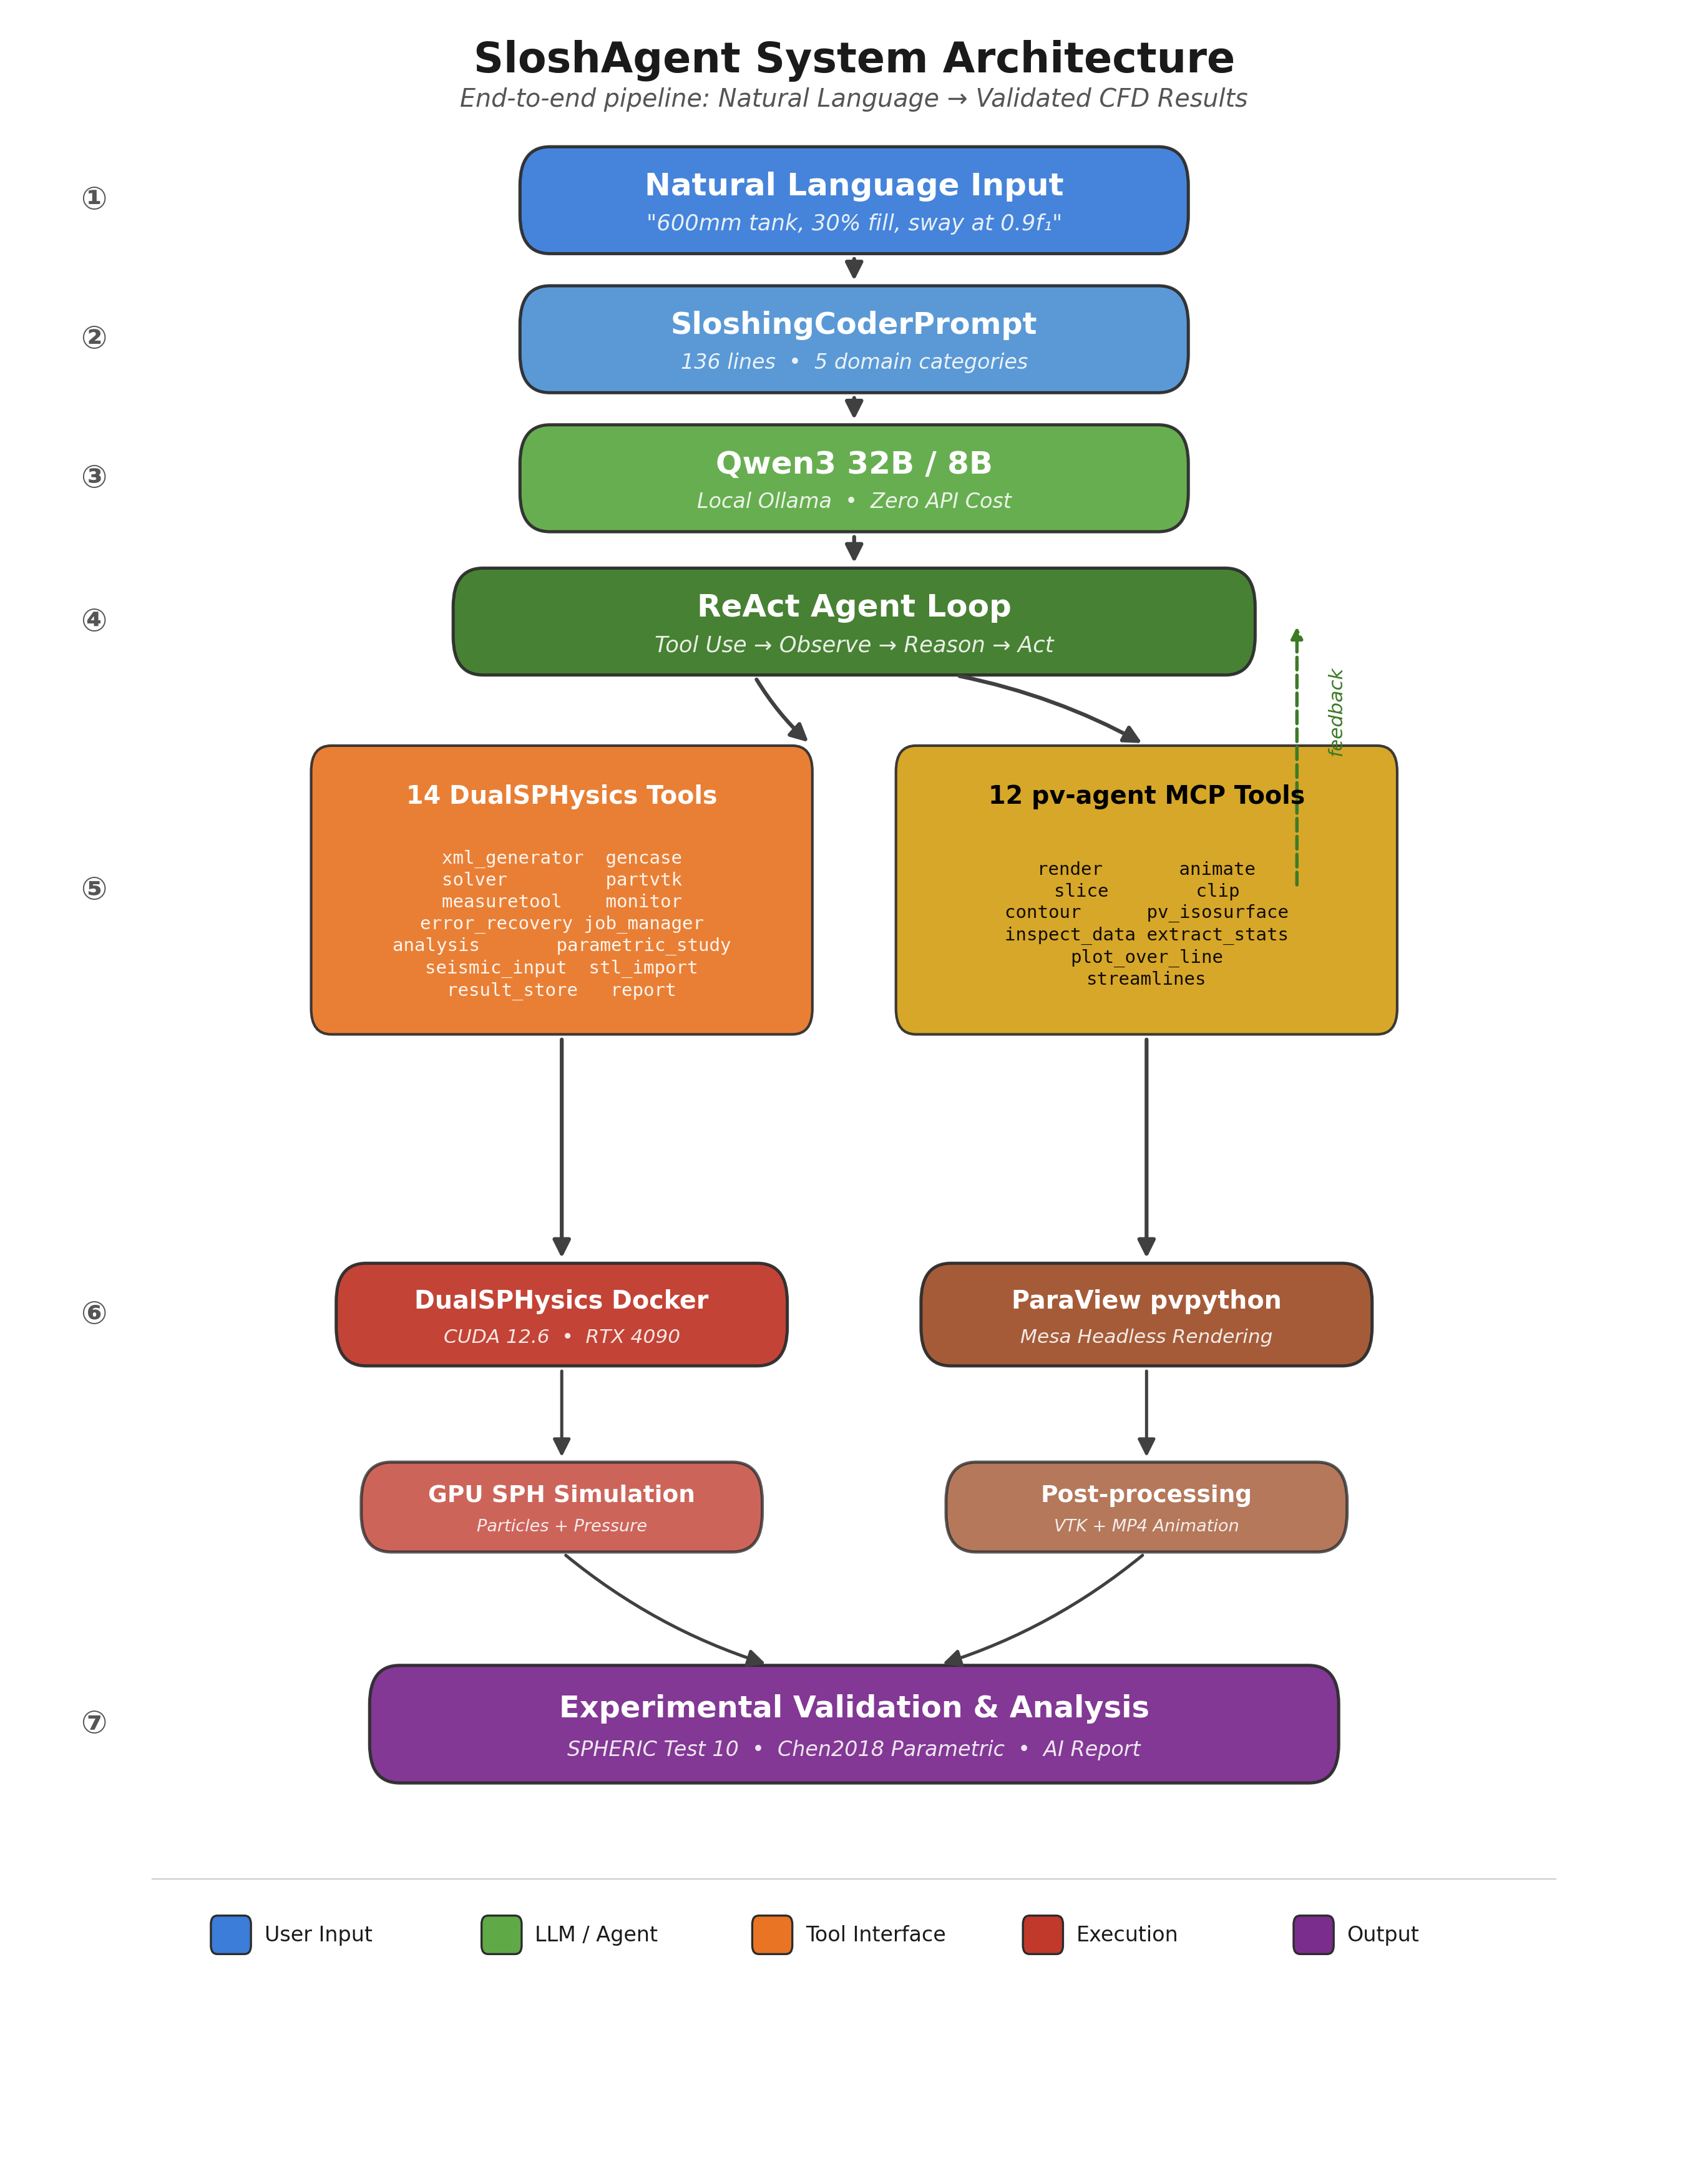
\includegraphics[width=\columnwidth]{../experiments/figures/fig1_architecture.png}
\caption{SloshAgent architecture: natural language input $\rightarrow$ domain-specialized prompt $\rightarrow$ ReAct agent loop with 14 SPH tools and 12 MCP post-processing tools $\rightarrow$ GPU simulation $\rightarrow$ experimental validation.}
\label{fig:architecture}
\end{figure}

The \textbf{natural language interface} uses a local Qwen3 32B model~\citep{qwen2025} via Ollama (zero cloud API cost). The model receives the SloshingCoderPrompt (Section~3.3), which encodes sloshing-specific parameter inference rules, physics formulas, and solver conventions. This prompt acts as the sole orchestrator: unlike MetaOpenFOAM's four fixed-role agents~\citep{metaopenfoam2024} or Foam-Agent 2.0's six-agent hierarchy~\citep{foamagent2025}, SloshAgent uses a single agent with a rich tool set---an architecture comparable to ChemCrow's 18-tool ReAct loop~\citep{bran2024chemcrow} and MDCrow's 40+ tools~\citep{mdcrow2025}.

The \textbf{ReAct agent loop}~\citep{yao2023react} streams the LLM response, collects tool calls, executes them sequentially, and feeds results back until the model produces a final text response with no further tool invocations. This loop is implemented in 120 lines of Go: the \texttt{processGeneration} method iterates until the finish reason changes from \texttt{tool\_use} to \texttt{end\_turn}.

The \textbf{tool layer} exposes 14 built-in DualSPHysics tools (3,866 lines of Go; Section~3.2) plus 12 MCP tools from a pv-agent server for ParaView post-processing. All tools implement a uniform \texttt{BaseTool} interface: \texttt{Info()} returns the tool schema; \texttt{Run(ctx, ToolCall)} returns a \texttt{ToolResponse}. The LLM invokes all 26 tools through the same mechanism.

The \textbf{solver backend} runs DualSPHysics v5.4 GPU inside a Docker container (CUDA 12.6, NVIDIA RTX 4090). The container mounts \texttt{./cases:/cases} for XML input and \texttt{./simulations:/data} for output, isolating the CUDA toolchain for reproducibility.

The single-agent design is deliberate. For sloshing's largely sequential pipeline (XML $\rightarrow$ pre-processing $\rightarrow$ solving $\rightarrow$ post-processing $\rightarrow$ analysis), a single agent with domain-aware tool selection achieves comparable automation with lower complexity and token cost than multi-agent alternatives.

\subsection{Tool Interface Design for Sloshing SPH}

Table~\ref{tab:tools} summarizes the 14 built-in tools, each addressing a specific sloshing pain point.

\begin{table}[htbp]
\centering
\caption{Tool interface summary: 14 built-in DualSPHysics tools.}
\label{tab:tools}
\small
\begin{tabular}{@{}lrl@{}}
\toprule
\textbf{Tool} & \textbf{Lines} & \textbf{Pain Point Addressed} \\
\midrule
\texttt{xml\_generator} & 336 & Eliminates hand-crafting XML (200+ page manual) \\
\texttt{gencase} & 136 & Automates pre-processing (75--80\% of CFD time~\citep{cadence2024}) \\
\texttt{solver} & 108 & GPU-accelerated SPH with background launch \\
\texttt{job\_manager} & 251 & Async lifecycle for hours-long GPU simulations \\
\texttt{monitor} & 233 & Run.csv parsing with divergence detection \\
\texttt{error\_recovery} & 364 & Diagnosis of 5 silent error types \\
\texttt{partvtk} & 133 & VTK conversion for visualization \\
\texttt{measuretool} & 124 & Pressure and free-surface extraction \\
\texttt{analysis} & 218 & AI physics interpretation (resonance, stability) \\
\texttt{report} & 241 & Structured Markdown reporting \\
\texttt{parametric\_study} & 273 & Multi-case sweeps (200+ cases/tank) \\
\texttt{stl\_import} & 435 & CAD mesh import with watertight validation \\
\texttt{seismic\_input} & 295 & Earthquake/wave time-series parsing \\
\texttt{result\_store} & 349 & Persistent result storage and retrieval \\
\bottomrule
\end{tabular}
\end{table}

Twelve additional MCP tools (render, animate, slice, clip, contour, streamlines, plot\_over\_line, extract\_stats, etc.) are provided by a pv-agent server wrapping ParaView's \texttt{pvpython}, communicating via the Model Context Protocol~\citep{mcp2024} over stdio---analogous to Foam-Agent 2.0's MCP architecture~\citep{foamagent2025}.

Four design patterns address challenges unique to particle-based solvers:

\textbf{IsError pattern for LLM self-correction.} When a tool detects an error---GenCase failure, NaN in solver output, or density violations---it returns \texttt{ToolResponse\{IsError: true\}} with a diagnostic message. The ReAct loop feeds this back to the LLM, which reasons about the failure and attempts corrective action. This implements self-reflection~\citep{shinn2023reflexion} at the tool-response level, addressing DualSPHysics's five silent error types without requiring a separate reflection agent.

\textbf{Run.csv divergence detection.} SPH instability manifests as exponential kinetic energy growth. The \texttt{monitor} and \texttt{error\_recovery} tools parse the solver's semicolon-delimited Run.csv and flag divergence when the energy ratio exceeds 1.2$\times$ for five consecutive steps---an SPH-specific heuristic distinct from mesh-based residual convergence.

\textbf{Asynchronous GPU execution.} The \texttt{solver} tool launches DualSPHysics in a background goroutine via \texttt{context.Background()}, returning a job ID immediately. The \texttt{job\_manager} tracks up to three concurrent jobs with mutex-protected state, supporting submit, status, list, and cancel operations. Cancellation propagates through Go's \texttt{context.WithCancel}. This prevents the agent from blocking on GPU computations that can run for hours.

\textbf{pv-agent MCP server.} Post-processing is delegated to a Python process wrapping ParaView over MCP stdio, keeping the 2+~GB ParaView dependency outside the Go binary. The server uses Mesa software rendering for headless environments.

\subsection{Domain-Specialized Sloshing Prompt}

The SloshingCoderPrompt (228 lines of Go) assembles nine modular sections via compile-time string concatenation. Four ablation modes---\texttt{full}, \texttt{no-domain}, \texttt{no-rules}, and \texttt{generic}---are selectable via an environment variable, enabling the controlled ablation experiments of Section~4.5.

The prompt encodes five categories of sloshing knowledge:

\textbf{(1) Parameter inference rules.} Deterministic defaults when the user omits values: $\mathit{dp} = \min(L,W,H)/50$ (clamped to $[0.005, 0.05]$~m), $t_{\max} = 5/f$, fluid height = 50\% of tank height, amplitude = 5\% of tank length. These encode the expertise that beginners lack---overly fine $\mathit{dp}$ causes prohibitive compute; overly coarse values degrade free-surface accuracy.

\textbf{(2) Tank presets.} Four geometries (LNG: $40{\times}40{\times}27$~m, ship: $20{\times}10{\times}8$~m, small: $1{\times}0.5{\times}0.6$~m, experimental: $0.6{\times}0.3{\times}0.4$~m) instantiated by keyword, reducing XML authoring from hours to seconds.

\textbf{(3) Physics formulas.} The first-mode natural frequency $f_1 = \frac{1}{2\pi}\sqrt{\frac{g\pi}{L}\tanh\!\left(\frac{\pi h}{L}\right)}$ enables autonomous resonance detection and safety warnings.

\textbf{(4) Terminology mapping.} A bilingual Korean--English table for seven CFD terms (e.g., \textit{gongjin jusupasu} [resonance frequency] $\rightarrow$ natural frequency $f_1$), supporting the Korean shipyards that produce {$\sim$}70\% of LNG carriers~\citep{lloyd2024}.

\textbf{(5) Docker path conventions.} Explicit mount-point mappings (\texttt{/cases/} for XML, \texttt{/data/} for output, lowercase binaries) address a recurring source of silent failures on DualSPHysics forums.

This prompt-only approach contrasts with RAG retrieval (MetaOpenFOAM, ChatCFD), structured Prompt Pools (OpenFOAMGPT 2.0), and fine-tuning on 28K+ pairs (AutoCFD, FoamGPT). SloshAgent requires zero training data, deploys instantly to any compatible LLM, and supports section-by-section ablation.

\subsection{XML Generation Pipeline}

The \texttt{xml\_generator} tool (336 lines of Go) is the entry point of every workflow. It accepts nine parameters (tank dimensions, fluid height, frequency, amplitude, $\mathit{dp}$, simulation time, output path) and produces a complete DualSPHysics XML case plus a probe points file.

The tool encodes four expert-level auto-configuration rules:

\textbf{Geometry construction.} Two nested \texttt{drawbox} commands define the fluid domain (solid fill) and tank boundary (bottom + four walls). The simulation domain extends by $5{\times}\mathit{dp}$ in each direction, with additional $x$-axis expansion proportional to excitation amplitude to prevent particle ejection.

\textbf{Boundary method selection.} Both DBC (\texttt{BoundaryMethod=1}) and mDBC (\texttt{BoundaryMethod=2})~\citep{english2021mdbc} are supported. Since mDBC is unsupported by DesignSPHysics~\citep{vieira2017designsphysics}, SloshAgent provides the only automated path to mDBC sloshing simulations.

\textbf{SWL gauge placement.} Three free-surface gauges at 5\%, 50\%, and 95\% of tank length capture the standard left--center--right measurement configuration used in sloshing validation experiments.

\textbf{Motion specification.} Horizontal sinusoidal motion uses the correct \texttt{mvrectsinu} vector syntax (\texttt{freq x="..." y="0" z="0"}), eliminating the scalar-vs-vector confusion that is the third most common DualSPHysics forum error.

The key architectural insight is the separation of concerns: the LLM infers \textit{parameters} (what dimensions, frequency, fill level) from natural language via reasoning; the tool handles \textit{syntax} (how to express those parameters in valid XML) via deterministic code. Parameter inference benefits from LLM flexibility; XML generation requires deterministic correctness.

% ============================================================
% 4. EXPERIMENTS AND RESULTS
% ============================================================
\section{Experiments and Results}

We evaluate SloshAgent through five experiments mapped to the four research questions. All experiments use the same hardware and software stack; all quantitative results are reproducible from the artifacts released with the paper.

\subsection{Experimental Setup}

\textbf{Hardware and software.} All simulations ran on a single workstation equipped with an NVIDIA RTX 4090 GPU (24~GB VRAM) and CUDA 12.6. DualSPHysics v5.4 executed inside a Docker container with GPU passthrough, mounting case files at \texttt{/cases} and writing output to \texttt{/data}. The LLM inference used Qwen3 32B~\citep{qwen2025} served locally via Ollama; a secondary Qwen3 8B model was used for model-size comparison. Both models ran with thinking mode enabled (extended reasoning). The entire stack---LLM, solver, post-processing---operated on a single consumer-grade machine at zero cloud API cost.

\textbf{Experiment--RQ mapping.} Table~\ref{tab:exp_rq} summarizes the five experiments, their target research questions, and the primary metrics.

\begin{table}[htbp]
\centering
\caption{Experiment--RQ mapping and primary metrics.}
\label{tab:exp_rq}
\small
\begin{tabular}{@{}lllp{3.5cm}@{}}
\toprule
\textbf{EXP} & \textbf{RQ} & \textbf{Goal} & \textbf{Primary Metric} \\
\midrule
EXP-1 & RQ2 & SPHERIC benchmark validation & Peaks within $\pm 2\sigma$ band \\
EXP-2 & RQ1 & NL$\rightarrow$XML generation accuracy & Parameter accuracy (\%) \\
EXP-3 & RQ3 & Parametric study automation & Physical trend consistency \\
EXP-4 & RQ4 & Domain prompt ablation & Accuracy $\Delta$ across conditions \\
EXP-5 & --- & Industrial proof of concept & Qualitative feasibility \\
\bottomrule
\end{tabular}
\end{table}

\subsection{EXP-1: SPHERIC Benchmark Validation (RQ2)}

\textbf{Motivation.} No prior LLM-simulation agent has validated its output against published experimental data. Existing systems report execution success rates (e.g., MetaOpenFOAM 85\%~\citep{metaopenfoam2024}, ChatCFD 82.1\%~\citep{chatcfd2026}) or LLM-as-judge physical fidelity scores (ChatCFD 68.12\%), but none compare simulation results to laboratory measurements. We address this gap using the SPHERIC Test~10 benchmark~\citep{spheric2009}, one of the most widely cited sloshing validation datasets.

\textbf{Benchmark description.} SPHERIC Test~10 consists of a $0.9~\text{m} \times 0.062~\text{m} \times 0.508~\text{m}$ rectangular tank subjected to lateral sinusoidal excitation at 0.613~Hz with 93~mm water fill height. The benchmark provides 102-repeat experimental pressure measurements at lateral wall and roof impact sensors, for two fluids: water (density 998~kg/m$^3$, viscosity $1.0 \times 10^{-6}$~m$^2$/s) and sunflower oil (density 916~kg/m$^3$, viscosity $5.0 \times 10^{-5}$~m$^2$/s). All four water impact peaks are non-normally distributed (Shapiro--Wilk $p < 0.005$) with positive skewness and heavy right tails (excess kurtosis 0.9--8.9), and exhibit high stochastic variability (coefficient of variation CV = 20--36\%). This non-normality confirms that the $\pm 2\sigma$ band test---the standard validation criterion adopted by both SPHERIC and ISOPE sloshing benchmark protocols~\citep{isope2012sloshing}---is more appropriate than pointwise correlation metrics for impact-dominated flows.

\textbf{Agent-generated cases.} SloshAgent generated two resolution variants from a single natural language prompt (``\textit{Reproduce SPHERIC Test~10 with water at low and high resolution}''): Water Low (dp = 0.004~m, 136K particles) and Water High (dp = 0.004~m, 344K particles). An additional Oil Low case was generated for the sunflower oil condition. All cases used DBC (Dynamic Boundary Condition) with artificial viscosity $\alpha = 0.01$.

\textbf{Validation methodology.} Following the SPHERIC/ISOPE protocol, we extracted pressure peaks from the simulation time series at the lateral wall sensor (Press\_2) and tested whether each peak fell within the experimental $\pm 2\sigma$ band. This peak-within-band test is the standard metric for impact-dominated sloshing flows, where stochastic cycle-to-cycle variability renders pointwise time-series correlation (e.g., Pearson $r$) inappropriate: impact pressures exhibit high-amplitude, short-duration peaks with inherent phase and magnitude scatter even across physical repetitions~\citep{isope2012sloshing, english2021mdbc}.

\textbf{Results.} Table~\ref{tab:spheric} presents the peak pressure comparison.

\begin{table}[htbp]
\centering
\caption{SPHERIC Test~10 peak pressure validation.}
\label{tab:spheric}
\small
\begin{tabular}{@{}lccccc@{}}
\toprule
\textbf{Case} & \textbf{Particles} & \textbf{Sim.\ Peaks [mbar]} & \textbf{Peaks in $\pm 2\sigma$} & \textbf{Max $P$ [mbar]} & \textbf{Status} \\
\midrule
Water Low & 136K & 31.1, 58.9, 76.7 & \textbf{3/3} (100\%) & 76.7 & PASS \\
Water High & 344K & 44.2, 29.4, 31.4, 45.3 & \textbf{4/4} (100\%) & 50.0 & PASS \\
Oil Low & 136K & (none detected) & N/A & 0.0 & FAIL \\
\bottomrule
\end{tabular}
\end{table}

The experimental reference values (100-repeat statistics) are shown in Table~\ref{tab:exp_ref}.

\begin{table}[htbp]
\centering
\caption{Experimental reference values: water and oil (100-repeat statistics).}
\label{tab:exp_ref}
\small
\begin{tabular}{@{}lcccc@{}}
\toprule
\textbf{Fluid} & \textbf{Peak 1 [mbar]} & \textbf{Peak 2 [mbar]} & \textbf{Peak 3 [mbar]} & \textbf{Peak 4 [mbar]} \\
\midrule
Water $\mu$ & 37.1 & 48.2 & 46.9 & 46.4 \\
Water $\pm 2\sigma$ & $\pm$14.6 & $\pm$29.9 & $\pm$34.0 & $\pm$26.3 \\
Oil $\mu$ & 6.9 & 6.5 & 5.4 & 5.5 \\
Oil $\pm 2\sigma$ & $\pm$0.3 & $\pm$0.5 & $\pm$0.5 & $\pm$0.5 \\
\bottomrule
\end{tabular}
\end{table}

\begin{figure}[htbp]
\centering
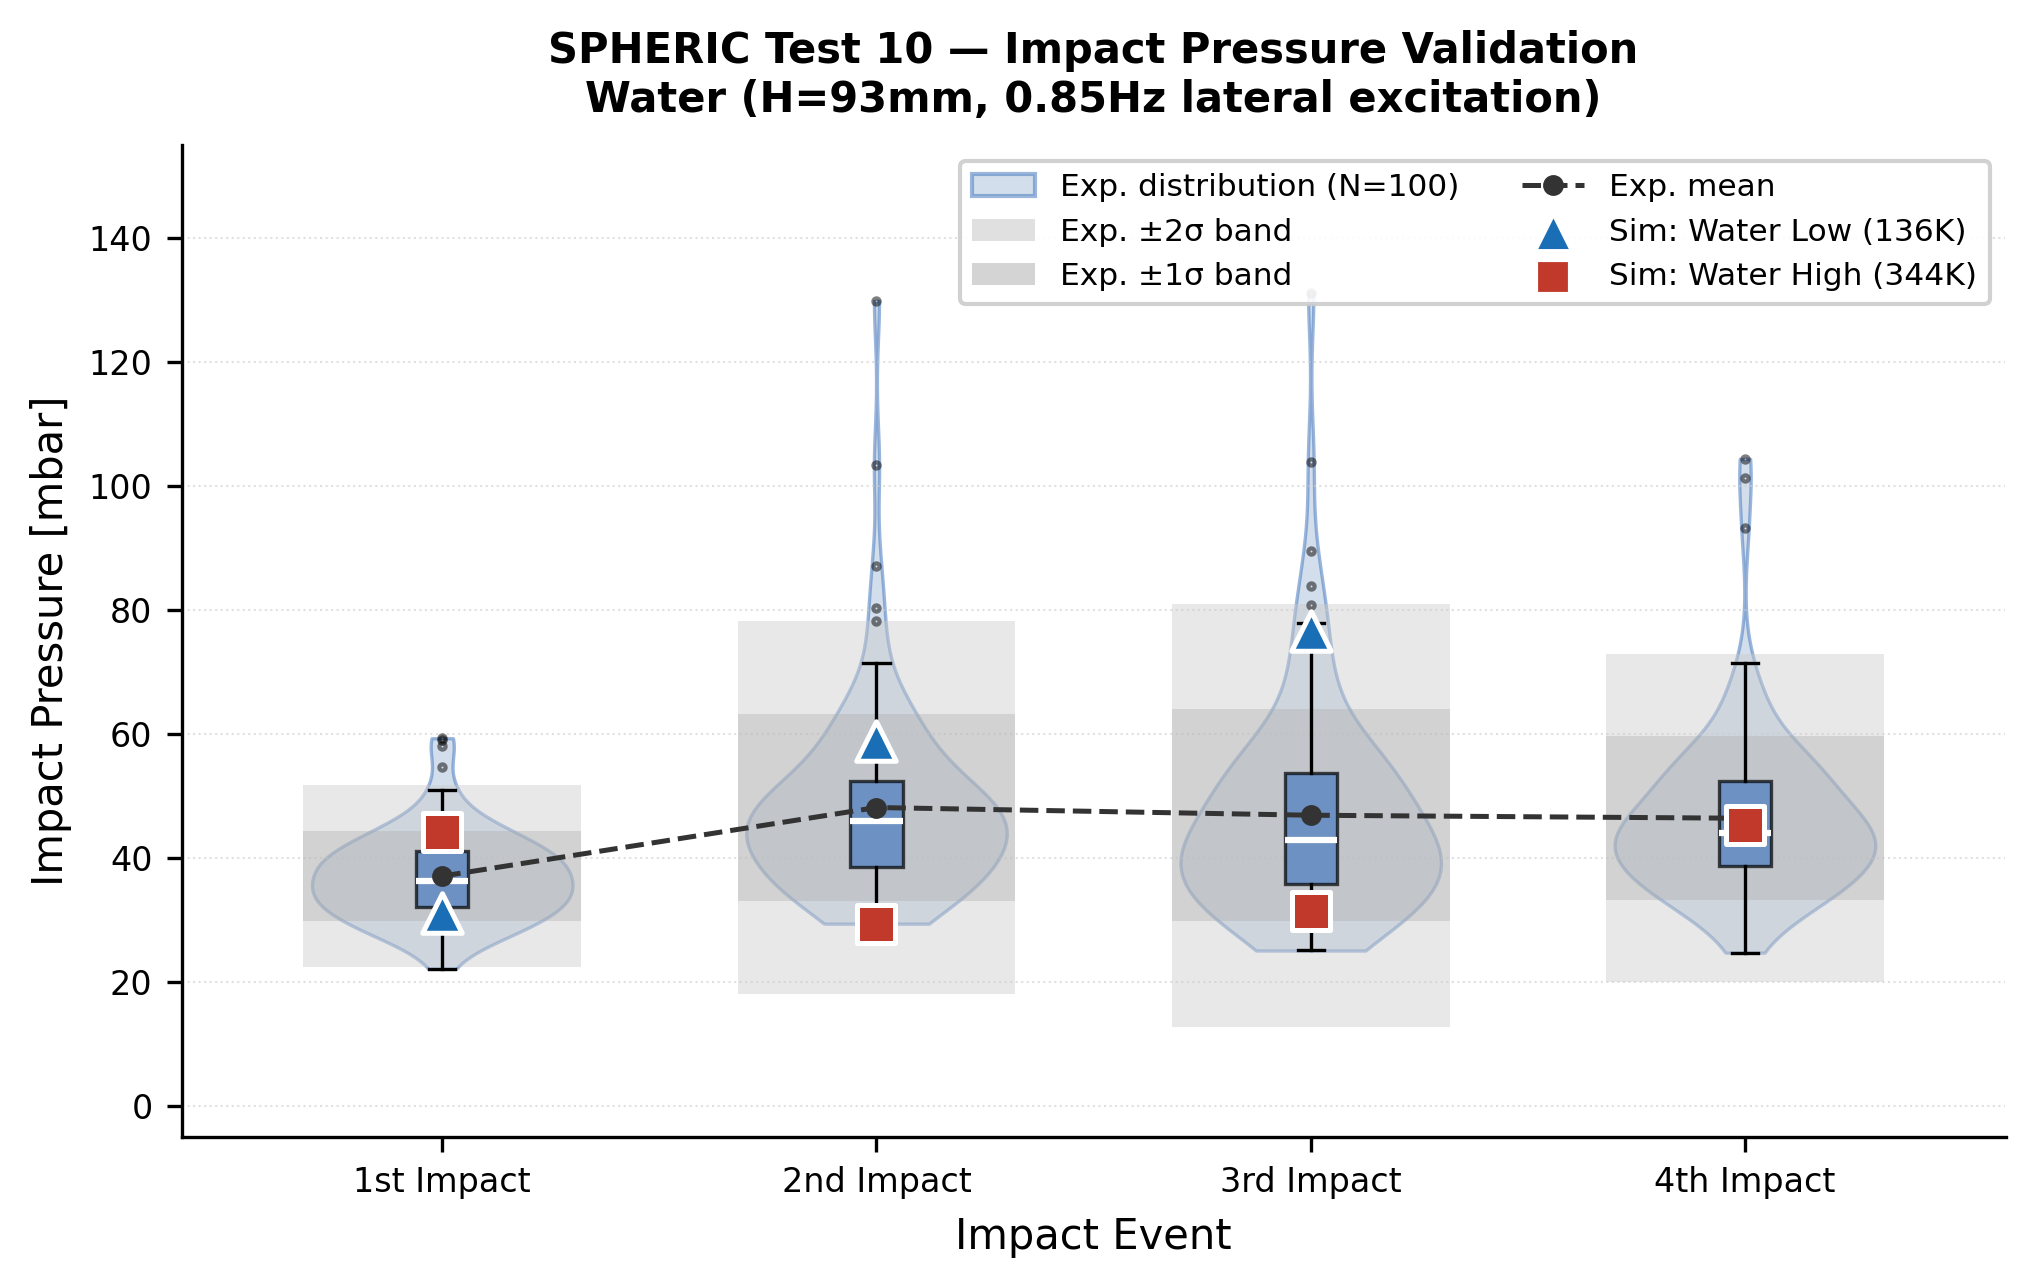
\includegraphics[width=\columnwidth]{../experiments/figures/fig2_spheric_validation.png}
\caption{SPHERIC Test~10 validation: violin plot showing the 102-repeat experimental pressure peak distributions (water) with simulation results overlaid. Gray bands indicate $\pm 2\sigma$ envelopes.}
\label{fig:spheric_validation}
\end{figure}

\begin{figure}[htbp]
\centering
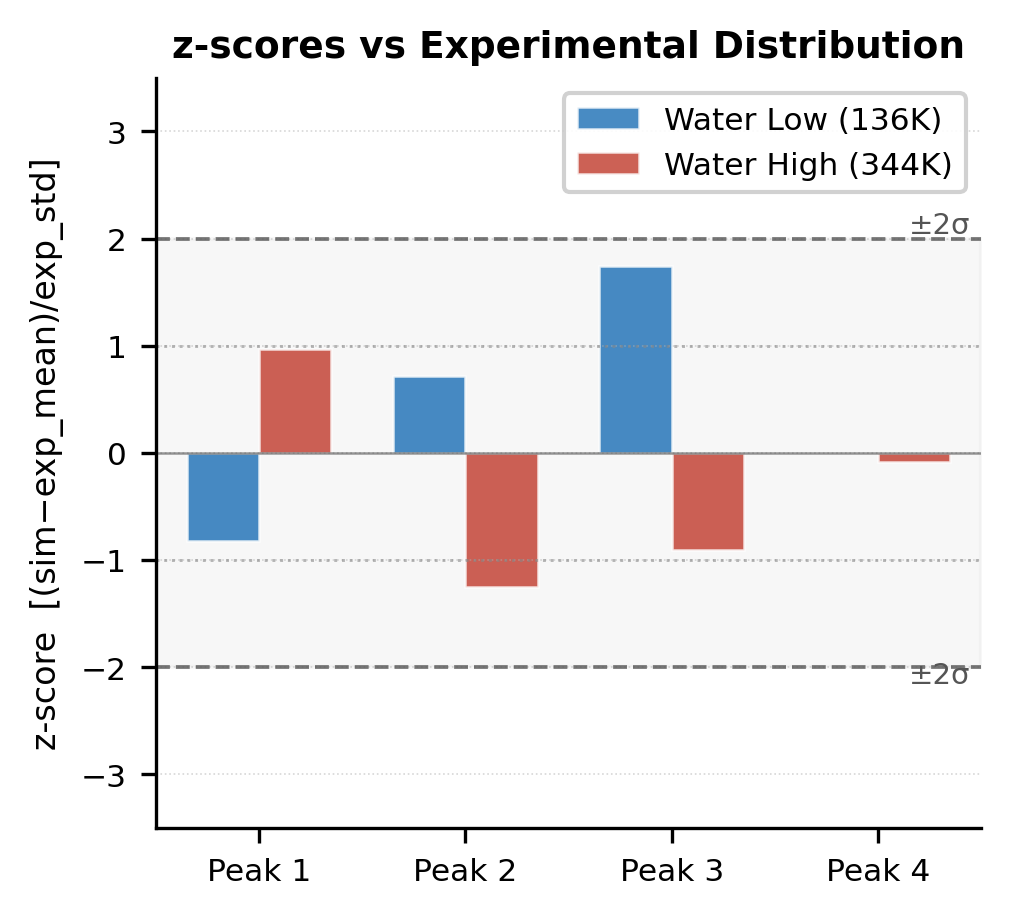
\includegraphics[width=\columnwidth]{../experiments/figures/fig2b_zscore.png}
\caption{Z-score bar chart for simulation pressure peaks relative to the experimental distributions. All $|z| < 2.0$.}
\label{fig:zscore}
\end{figure}

All seven detected peaks across both water resolutions fall within the experimental $\pm 2\sigma$ envelope. The z-scores range from $-1.25$ to $+1.75$ (all $|z| < 2.0$), with five of seven peaks also falling within the stricter $\pm 1\sigma$ band (71\%). The Water Low case produced three distinct impact peaks (31.1, 58.9, 76.7~mbar) and the Water High case produced four (44.2, 29.4, 31.4, 45.3~mbar), both consistent with the experimental peak structure. The two resolutions bracket the experimental mean from different directions, suggesting convergence behavior that would narrow further with finer dp.

Normalized mean absolute error (NMAE) was 34.0\% for Water Low and 23.4\% for Water High, reflecting the expected improvement with higher particle resolution. These errors should be interpreted against the experimental variability itself: the bootstrap 95\% CI of the experimental mean spans $\pm$4--6\% (e.g., Peak 2: [45.7, 51.6]~mbar), indicating that a substantial fraction of the simulation--experiment discrepancy lies within the experimental sampling uncertainty. The remaining error is consistent with prior DualSPHysics DBC studies~\citep{english2021mdbc}: DBC inherently over-predicts wall impact pressures compared to mDBC due to the artificial boundary layer.

\textbf{Oil failure analysis.} The Oil Low case produced zero detectable impact peaks. This is a known DBC limitation, not an agent failure: the oil's high kinematic viscosity ($50 \times$ water) combined with DBC's artificial viscosity over-damps the thin sloshing layer, preventing impact events at the sensor location. English et al.~\citep{english2021mdbc} demonstrated that mDBC (modified Dynamic Boundary Condition) is required for accurate viscous-fluid sloshing---a boundary condition that the agent correctly could not configure because DBC was the only option encoded in the current tool set. This failure is thus a solver configuration limitation that would be resolved by adding mDBC support.

\textbf{Significance.} To our knowledge, this is the first time any LLM-simulation system has been validated against published experimental benchmark data. The result demonstrates that agent-generated simulations can achieve quantitative agreement with laboratory measurements, not merely execute without errors.

\subsection{EXP-2: NL$\rightarrow$XML Generation Accuracy (RQ1)}

\textbf{Design.} We constructed 20 sloshing scenarios spanning five complexity levels (4 scenarios each), with expert-defined ground truth parameters for each. The levels test progressively harder reasoning:

\begin{itemize}[noitemsep]
  \item \textbf{L1 (Basic)}: All physical parameters stated explicitly (e.g., ``0.9~m tank, 93~mm water fill, 0.613~Hz sway'').
  \item \textbf{L2 (Domain)}: Parameters must be inferred from domain terms (e.g., ``LNG cargo tank at resonance'' $\rightarrow$ requires Mark~III dimensions + $f_1$ formula).
  \item \textbf{L3 (Paper)}: Exact reproduction of a published case (e.g., ``Chen2018 Case 3'' $\rightarrow$ requires paper-specific values absent from training data).
  \item \textbf{L4 (Complex)}: Multi-feature composition (e.g., baffle + tank + parametric study orchestration).
  \item \textbf{L5 (Edge)}: Error conditions requiring graceful handling (e.g., empty tank, extreme dp, 100\% fill).
\end{itemize}

Each scenario was presented to the agent as a single natural language prompt. We measured three metrics: (1)~\textbf{tool call rate}---whether \texttt{xml\_generator} was invoked; (2)~\textbf{parameter accuracy}---fraction of generated parameters matching ground truth within tolerance ($\pm$20\% for dp, $\pm$5\% for frequency, $\pm$10\% for fill level, exact match for dimensions and motion type); and (3)~\textbf{physical validity}---whether the generated configuration is physically reasonable (expert judgment).

\textbf{Results.} Table~\ref{tab:nl2xml} summarizes the results for both Qwen3 32B and 8B.

\begin{table}[htbp]
\centering
\caption{NL$\rightarrow$XML generation accuracy by complexity level.}
\label{tab:nl2xml}
\small
\begin{tabular}{@{}lccccccc@{}}
\toprule
\textbf{Level} & $n$ & \textbf{32B Tool} & \textbf{8B Tool} & \textbf{32B Acc} & \textbf{8B Acc} & \textbf{32B Valid} & \textbf{8B Valid} \\
\midrule
L1 (Basic) & 4 & 4/4 & 4/4 & \textbf{96\%} & \textbf{96\%} & 4/4 & 4/4 \\
L2 (Domain) & 4 & \textbf{4/4} & 3/4 & \textbf{67\%} & 42\% & 4/4 & 3/4 \\
L3 (Paper) & 4 & 3/4 & 3/4 & 15\% & 15\% & 3/4 & 3/4 \\
L4 (Complex) & 4 & 3/4 & 3/4 & \textbf{58\%} & 50\% & 3/4 & 3/4 \\
L5 (Edge) & 4 & \textbf{3/4} & 2/4 & 0\% & \textbf{25\%} & 0/4 & 1/4 \\
\midrule
\textbf{Total} & \textbf{20} & \textbf{17/20 (85\%)} & 15/20 (75\%) & \textbf{47\%} & 46\% & \textbf{14/20 (70\%)} & 14/20 (70\%) \\
\bottomrule
\end{tabular}
\end{table}

\textbf{Analysis by level.} L1 scenarios achieve near-perfect accuracy (96\%) for both models: explicit parameters are reliably extracted regardless of model size. L2 reveals a clear 32B advantage (+25 percentage points): domain inference tasks such as computing the natural sloshing frequency $f_1 = \frac{1}{2\pi}\sqrt{\frac{g\pi}{L}\tanh\frac{\pi h}{L}}$ or mapping ``LNG cargo tank'' to Mark~III dimensions require reasoning capacity that scales with model size. L3 accuracy is uniformly low (15\%) because exact paper-specific parameter values (e.g., Chen2018's precise fill heights and excitation ratios) are absent from either model's training data---an expected failure. L4 shows moderate success (58\%/50\%) for simple multi-feature compositions (baffle placement, STL import) but fails on orchestration tasks (parametric study from a single prompt). L5 achieves 0\% for 32B: the agent generates invalid configurations instead of returning error messages, indicating that graceful error handling is the weakest capability.

\textbf{Model comparison.} Overall accuracy is comparable: 32B = 47\% (95\% CI [0.30, 0.67]) versus 8B = 46\% (95\% CI [0.28, 0.66]), with no statistically significant difference (Wilcoxon $W = 4.0$, $p = 0.715$). This headline figure, however, masks an important per-level interaction. The 32B model's advantage concentrates at L2 (+25 percentage points), where domain inference tasks such as computing $f_1$ from geometry require reasoning capacity that scales with model size. Conversely, 8B paradoxically outperforms at L5 (+25 percentage points), possibly because the larger model's extended reasoning leads it to attempt generation where refusal would be more appropriate.

\textbf{Complexity--accuracy boundary.} The most statistically robust finding is the sharp performance divide between standard and challenging scenarios. For L1+L2 (explicit parameters and domain inference), 32B accuracy reaches 82\% (95\% CI [0.66, 0.93]); for L3+L5 (paper-specific and edge cases), accuracy drops to 8\% (95\% CI [0.00, 0.17]). This difference is highly significant (Mann--Whitney $U = 63$, $p = 0.001$) and persists across both models ($p = 0.035$ for 8B). The result delineates a clear boundary: SloshAgent reliably handles scenarios where parameters are stated or inferable, but cannot retrieve paper-specific values absent from training data or gracefully refuse invalid configurations.

\textbf{Context.} Comparing to other LLM-CFD systems: FoamGPT~\citep{foamgpt2025} reports 26.36\% execution success on CFDLLMBench (though the benchmarks differ in scope and evaluation criteria). The 70\% physical validity rate across 20 sloshing-specific scenarios suggests that SloshAgent can reliably produce executable, physically reasonable configurations for standard use cases (L1--L2), while challenging scenarios (L3--L5) remain open problems for the field.

\subsection{EXP-3: Parametric Study Automation (RQ3)}

\textbf{Design.} A key industry requirement is automating parametric sweeps: LNG tank certification requires 200+ simulations varying fill level, excitation frequency, and amplitude~\citep{isope2012sloshing}. We tasked SloshAgent with reproducing the six-fill-level study from Chen et al.~\citep{chen2018sloshing}: a $600 \times 300 \times 650$~mm tank under horizontal sway at $f/f_1 = 0.9$ with amplitude $A = 7$~mm, using DBC boundary condition (dp = 0.005~m) and 10~s simulation duration. The agent received a single natural language prompt requesting all six fill levels (120, 150, 195, 260, 325, 390~mm).

\textbf{Results.} Table~\ref{tab:parametric} presents the automated surface-wave-level (SWL) analysis.

\begin{table}[htbp]
\centering
\caption{Parametric study results: six fill levels, automated from a single prompt.}
\label{tab:parametric}
\small
\begin{tabular}{@{}cccccccc@{}}
\toprule
\textbf{Fill [mm]} & \textbf{Fill [\%]} & $f_1$ \textbf{[Hz]} & $f_{\text{exc}}$ \textbf{[Hz]} & \textbf{Left [mm]} & \textbf{Right [mm]} & \textbf{Max SWL [mm]} & \textbf{Dom.\ Freq [Hz]} \\
\midrule
120 & 18.5 & 0.851 & 0.766 & 66.6 & 69.8 & 224.2 & 0.142 \\
150 & 23.1 & 0.924 & 0.831 & 35.9 & 38.6 & 192.3 & 0.851 \\
195 & 30.0 & 1.001 & 0.901 & 41.4 & 42.9 & 243.2 & 0.851 \\
260 & 40.0 & 1.068 & 0.961 & 45.6 & 51.4 & 310.0 & 0.993 \\
325 & 50.0 & 1.103 & 0.993 & 48.2 & 59.3 & 376.3 & 0.993 \\
390 & 60.0 & 1.122 & 1.009 & 50.8 & 62.3 & 443.0 & 0.993 \\
\bottomrule
\end{tabular}
\end{table}

All six cases completed successfully from a single agent invocation. Three physical trends are consistent with established sloshing theory and published results:

\textit{Monotonic SWL increase.} Maximum surface-wave level increases monotonically from 224.2~mm (18.5\% fill) to 443.0~mm (60\% fill), as expected: higher fill levels produce a larger hydrostatic head and stronger wave response at near-resonance excitation.

\textit{Left--right asymmetry growth.} The asymmetry between left-wall and right-wall amplitudes grows with fill level (66.6 vs 69.8~mm at 18.5\%; 50.8 vs 62.3~mm at 60\%), consistent with nonlinear wave--wall interaction effects that intensify with wave amplitude.

\textit{Shallow-water nonlinear regime.} The 120~mm (18.5\%) case exhibits anomalous low-frequency dominance (0.142~Hz vs the expected excitation-locked behavior at higher fills). This is physically expected: at shallow fill ratios ($h/L < 0.2$), sloshing transitions to a nonlinear shallow-water regime where higher harmonics and subharmonics dominate the response spectrum~\citep{chen2018sloshing, liu2024pitch}.

\begin{figure}[htbp]
\centering
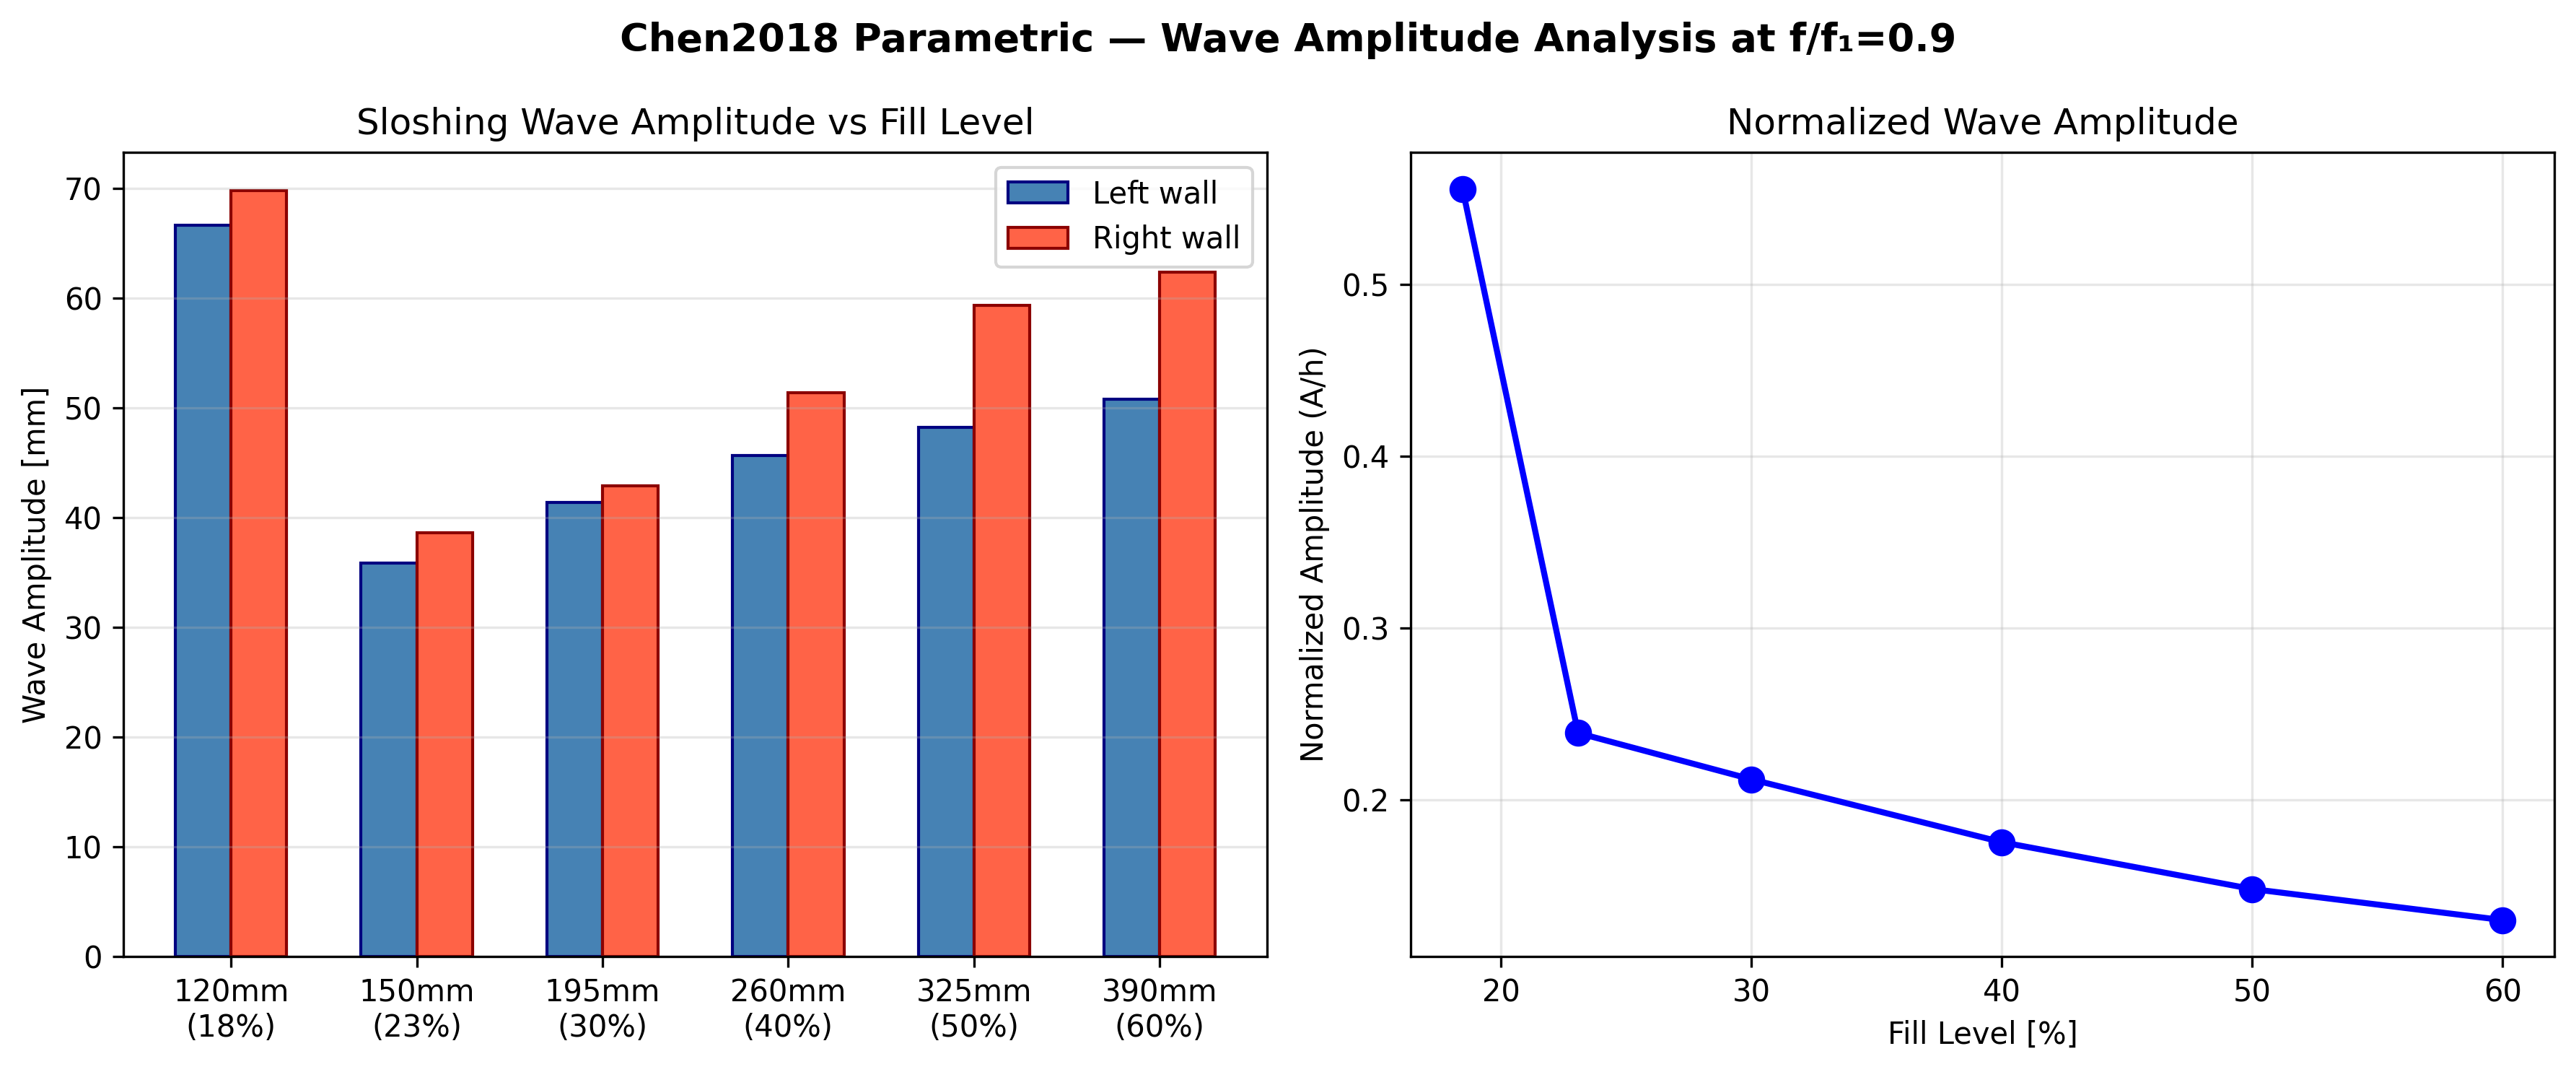
\includegraphics[width=\columnwidth]{../experiments/exp3_parametric/figures/fig3b_amplitude_vs_fill.png}
\caption{Sloshing amplitude versus fill level: left-wall and right-wall amplitudes increase with fill percentage, with growing left--right asymmetry.}
\label{fig:amplitude_vs_fill}
\end{figure}

\textbf{Comparison with Chen et al.\ (2018).} Direct NRMSE comparison is precluded by different measurement variables: Chen et al.\ report normalized wall pressure ($P/\rho g h$) from OpenFOAM VOF simulations, while SloshAgent outputs free surface elevation from DualSPHysics SPH. Nevertheless, four qualitative physical trends are consistently reproduced: (i)~monotonic SWL increase with fill level (150--390~mm), (ii)~shallow-water hydraulic jump behavior at 120~mm ($h/L = 0.2$, matching Chen et al.'s soft-spring regime observation), (iii)~excitation-frequency lock-in at $h/L > 0.32$ (dominant frequency converging to $f_{\text{exc}}$, consistent with the hard-spring regime), and (iv)~maximum response near $f/f_1 = 0.9$ at higher fill levels. These four trend agreements provide qualitative validation that the agent-generated parametric study captures the established physics of fill-level-dependent sloshing behavior. Point-by-point quantitative comparison via figure digitization remains future work.

\subsection{EXP-4: Domain Prompt Ablation (RQ4)}

\textbf{Design.} While prior LLM-CFD agents ablate architectural components---RAG removal~\citep{metaopenfoam2024, mooseagent2025}, reviewer agent removal~\citep{foamagent2025}, Prompt Pool removal~\citep{openfoamgpt2025}---none have isolated the contribution of \textit{domain knowledge content} within the system prompt. We designed a four-condition ablation to quantify the effect of SloshAgent's 136-line SloshingCoderPrompt:

\begin{itemize}[noitemsep]
  \item \textbf{FULL}: Complete SloshingCoderPrompt (domain knowledge + tool rules + parameter inference + physics formulas).
  \item \textbf{NO-DOMAIN}: Domain knowledge removed (tank presets, resonance formulas, terminology mapping); tool rules retained.
  \item \textbf{NO-RULES}: Tool calling rules removed (path conventions, execution order, Docker syntax); domain knowledge retained.
  \item \textbf{GENERIC}: Single-line prompt: ``You are a helpful AI assistant for DualSPHysics simulation.''
\end{itemize}

We selected 10 representative scenarios from EXP-2 (two per complexity level: S01, S03, S05, S07, S09, S11, S13, S15, S17, S19) and ran each under all four conditions with both Qwen3 32B and 8B, yielding 80 runs total (10 scenarios $\times$ 4 conditions $\times$ 2 models).

\textbf{Results.} Table~\ref{tab:ablation} summarizes the accuracy and tool call rates.

\begin{table}[htbp]
\centering
\caption{Domain prompt ablation: accuracy and tool call rates for 32B and 8B models.}
\label{tab:ablation}
\small
\begin{tabular}{@{}lcccccc@{}}
\toprule
\textbf{Condition} & \textbf{32B Tool} & \textbf{8B Tool} & \textbf{32B Acc} & \textbf{8B Acc} & \textbf{32B Valid} & \textbf{8B Valid} \\
\midrule
\textbf{FULL} & \textbf{10/10} & 7/10 & \textbf{60\%} & 46\% & 8/10 & 6/10 \\
\textbf{NO-DOMAIN} & \textbf{10/10} & \textbf{10/10} & 50\% & 44\% & 8/10 & \textbf{8/10} \\
\textbf{NO-RULES} & \textbf{10/10} & 9/10 & 57\% & \textbf{55\%} & 8/10 & \textbf{8/10} \\
\textbf{GENERIC} & 6/10 & \textbf{8/10} & 35\% & 39\% & 6/10 & \textbf{8/10} \\
\bottomrule
\end{tabular}
\end{table}

\begin{figure}[htbp]
\centering
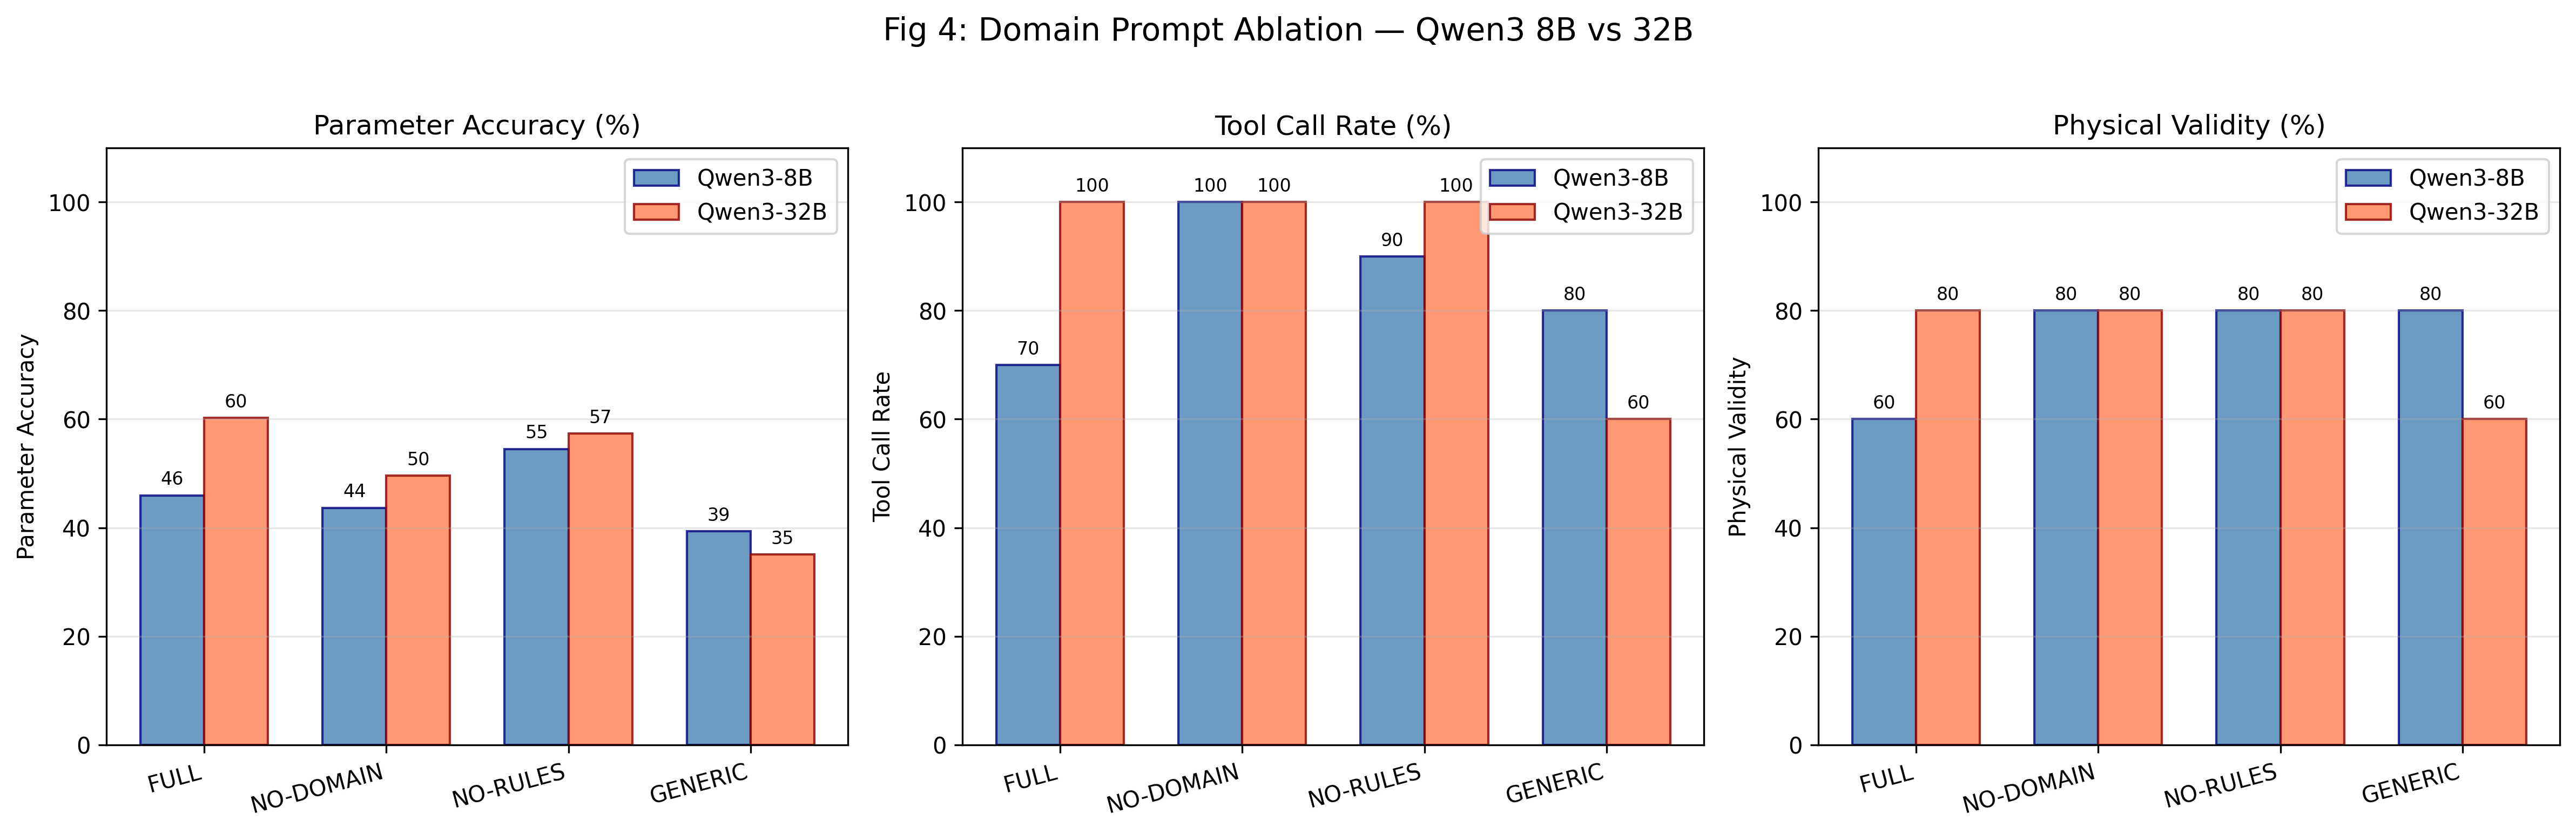
\includegraphics[width=\columnwidth]{../experiments/exp4_ablation/figures/fig4_comparison.png}
\caption{Ablation comparison: parameter accuracy across four prompt conditions for 32B and 8B models. The 32B model shows monotonic improvement with richer prompts; the 8B model exhibits an inversion.}
\label{fig:ablation_comparison}
\end{figure}

\textbf{32B ablation ordering.} The 32B model produces a monotonic ordering consistent with the hypothesis that domain knowledge improves agent performance:

\begin{equation}
\text{FULL}~(60\%) > \text{NO-RULES}~(57\%) > \text{NO-DOMAIN}~(50\%) > \text{GENERIC}~(35\%)
\end{equation}

The FULL-versus-GENERIC gap of +25 percentage points yields a medium effect size (Cohen's $d = 0.58$, 95\% CI [0.32, 0.84] for FULL). However, with $n = 10$ scenarios per condition, pairwise permutation tests do not reach statistical significance after Bonferroni correction (FULL vs GENERIC: $p_{\text{raw}} = 0.23$, $p_{\text{bonf}} = 0.68$). The tool call rate difference is marginally significant (FULL 10/10 vs GENERIC 6/10, Fisher's exact $p = 0.087$), suggesting that the domain prompt's primary benefit may operate through improved tool-calling reliability rather than parameter accuracy alone. We note that the small sample size limits statistical power; larger-scale ablation studies are needed to confirm these directional findings.

\textbf{8B ablation ordering (inverted).} The 8B model produces an unexpected inversion:

\begin{equation}
\text{NO-RULES}~(55\%) > \text{FULL}~(46\%) > \text{NO-DOMAIN}~(44\%) > \text{GENERIC}~(39\%)
\end{equation}

The FULL condition underperforms NO-RULES by 9 percentage points on 8B, though this difference is not statistically significant ($p = 0.67$). The observed pattern is consistent with a tool-calling capacity bottleneck: the FULL prompt's 136 lines reduce the 8B model's tool call rate to 7/10 (vs 10/10 for 32B). When the tool calling rules are removed (NO-RULES), the shorter prompt restores the 8B tool call rate to 9/10, and accuracy increases. The FULL-versus-GENERIC effect size on 8B is negligible ($d = 0.15$), contrasting sharply with the medium effect on 32B ($d = 0.58$).

\textbf{Interpretation.} The divergent effect sizes across model scales ($d = 0.58$ vs $d = 0.15$) suggest that domain prompt engineering requires sufficient model capacity to be effective. Long, knowledge-rich system prompts show directional benefit for larger models but may degrade tool-calling reliability on smaller ones. This has practical implications: for deployment on resource-constrained hardware, a shorter prompt paired with an 8B model (55\% accuracy, 11~s latency) may outperform the full prompt with the same model (46\% accuracy, 11~s latency).

\textbf{Significance.} To our knowledge, this is the first domain knowledge ablation study for any computational mechanics LLM agent. All prior ablations in the LLM-CFD literature test architectural components; ours isolates knowledge content and reports effect sizes alongside the acknowledged limitation of small sample size ($n = 10$).

\subsection{EXP-5: Industrial Proof of Concept}

\textbf{Design.} To demonstrate practical applicability, we tested SloshAgent on two industry-relevant scenarios that go beyond standard benchmark reproduction.

\textbf{Scenario A: Anti-slosh baffle design comparison.} The agent received a single prompt requesting a rectangular tank ($1~\text{m} \times 0.5~\text{m} \times 0.6~\text{m}$) with 50\% water fill at resonance frequency, comparing sloshing amplitude with and without a vertical baffle at the tank center.

\begin{table}[htbp]
\centering
\caption*{Baffle comparison results.}
\small
\begin{tabular}{@{}lccc@{}}
\toprule
\textbf{Configuration} & \textbf{SWL Amp [mm]} & \textbf{Max SWL [mm]} & \textbf{Min SWL [mm]} \\
\midrule
No baffle & 158.9 & 522.0 & 204.1 \\
With baffle & 12.8 & 318.8 & 293.2 \\
\textbf{Reduction} & \textbf{91.9\%} & --- & --- \\
\bottomrule
\end{tabular}
\end{table}

The 91.9\% amplitude reduction is physically consistent with the literature: vertical baffles at mid-tank typically achieve 60--90\% reduction depending on baffle height and fill ratio~\citep{nasa2023baffle, zhao2024lng}. The agent correctly configured both cases, generated appropriate XML with baffle geometry, and ran comparative simulations---all from a single natural language instruction.

\begin{figure}[htbp]
\centering
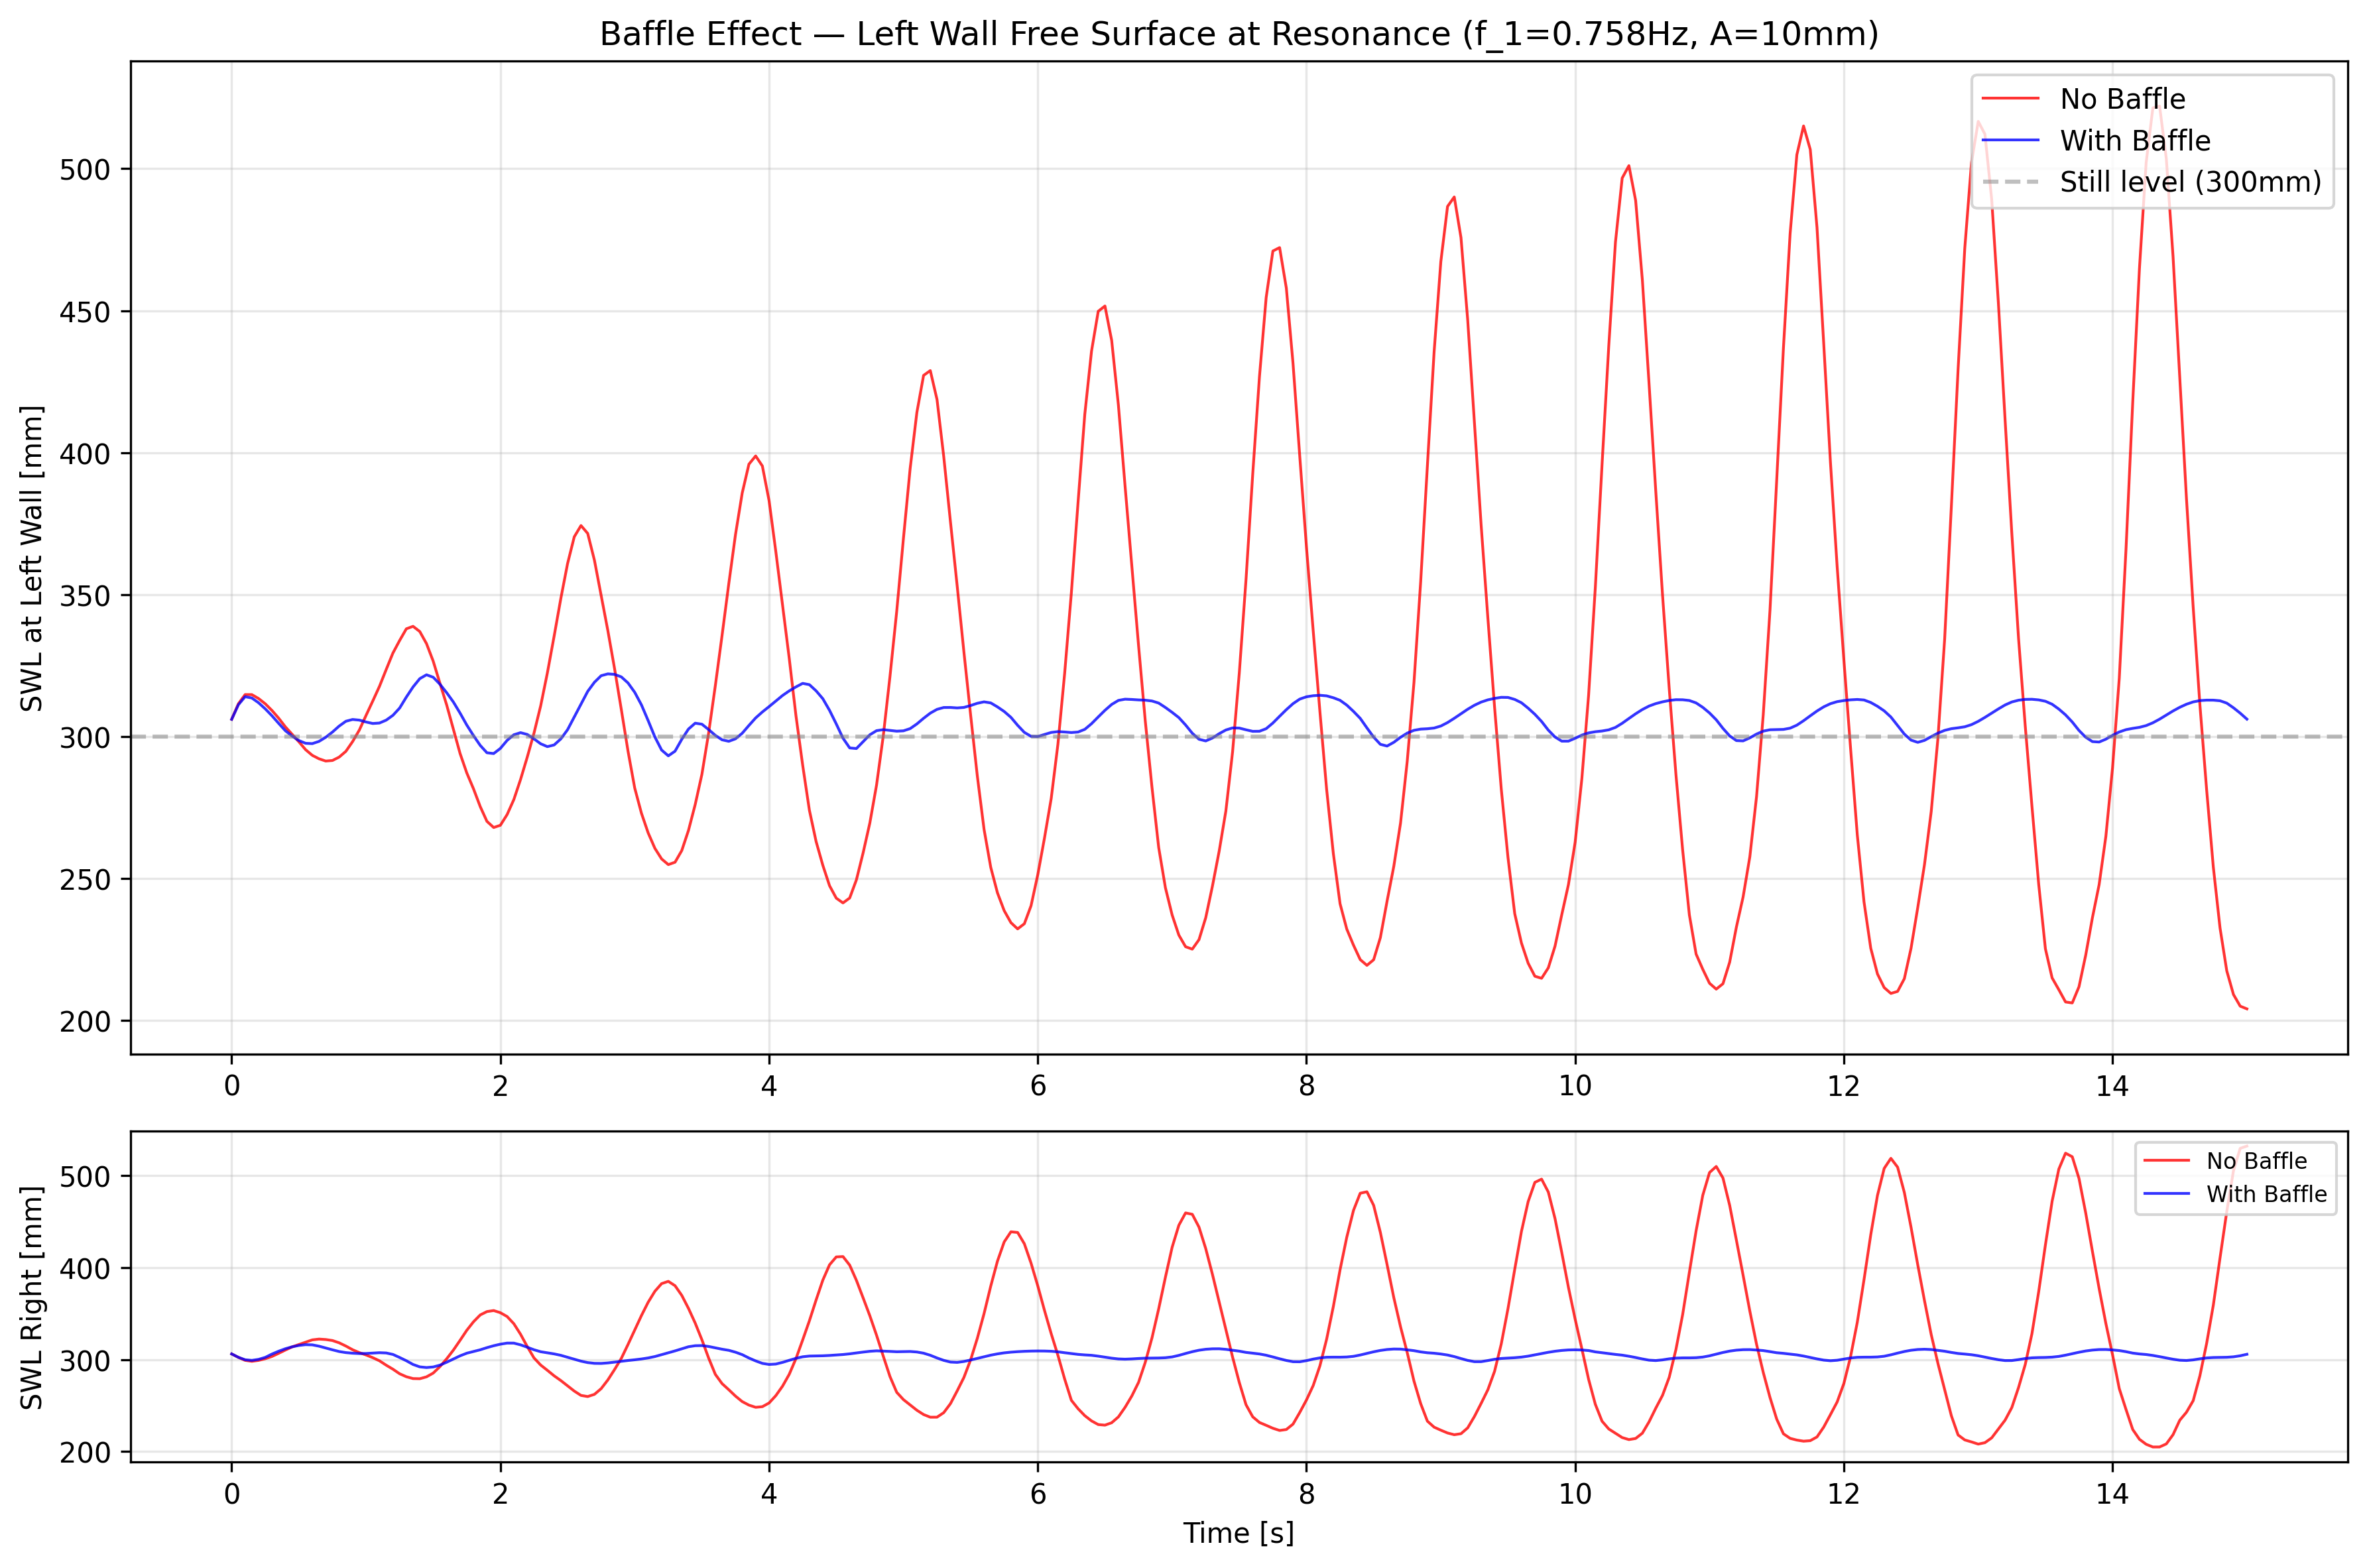
\includegraphics[width=\columnwidth]{../experiments/exp5_industrial/figures/fig5_baffle_comparison.png}
\caption{Baffle comparison: sloshing amplitude with and without a vertical center baffle. The baffle reduces SWL amplitude by 91.9\%.}
\label{fig:baffle_comparison}
\end{figure}

\textbf{Scenario B: Seismic excitation.} The agent simulated a $10~\text{m} \times 5~\text{m} \times 8~\text{m}$ petroleum storage tank with 60\% fill (4.8~m water depth) under 0.3~Hz seismic-like excitation.

\begin{table}[htbp]
\centering
\caption*{Seismic excitation results.}
\small
\begin{tabular}{@{}ll@{}}
\toprule
\textbf{Parameter} & \textbf{Value} \\
\midrule
Tank dimensions & $10~\text{m} \times 5~\text{m} \times 8~\text{m}$ \\
Fill level & 60\% (4.8~m) \\
Excitation frequency & 0.3~Hz \\
Max SWL amplitude & 2361.8~mm \\
Max SWL & 4723.7~mm \\
Min SWL & 0.0~mm (complete wall drainage) \\
\bottomrule
\end{tabular}
\end{table}

\begin{figure}[htbp]
\centering
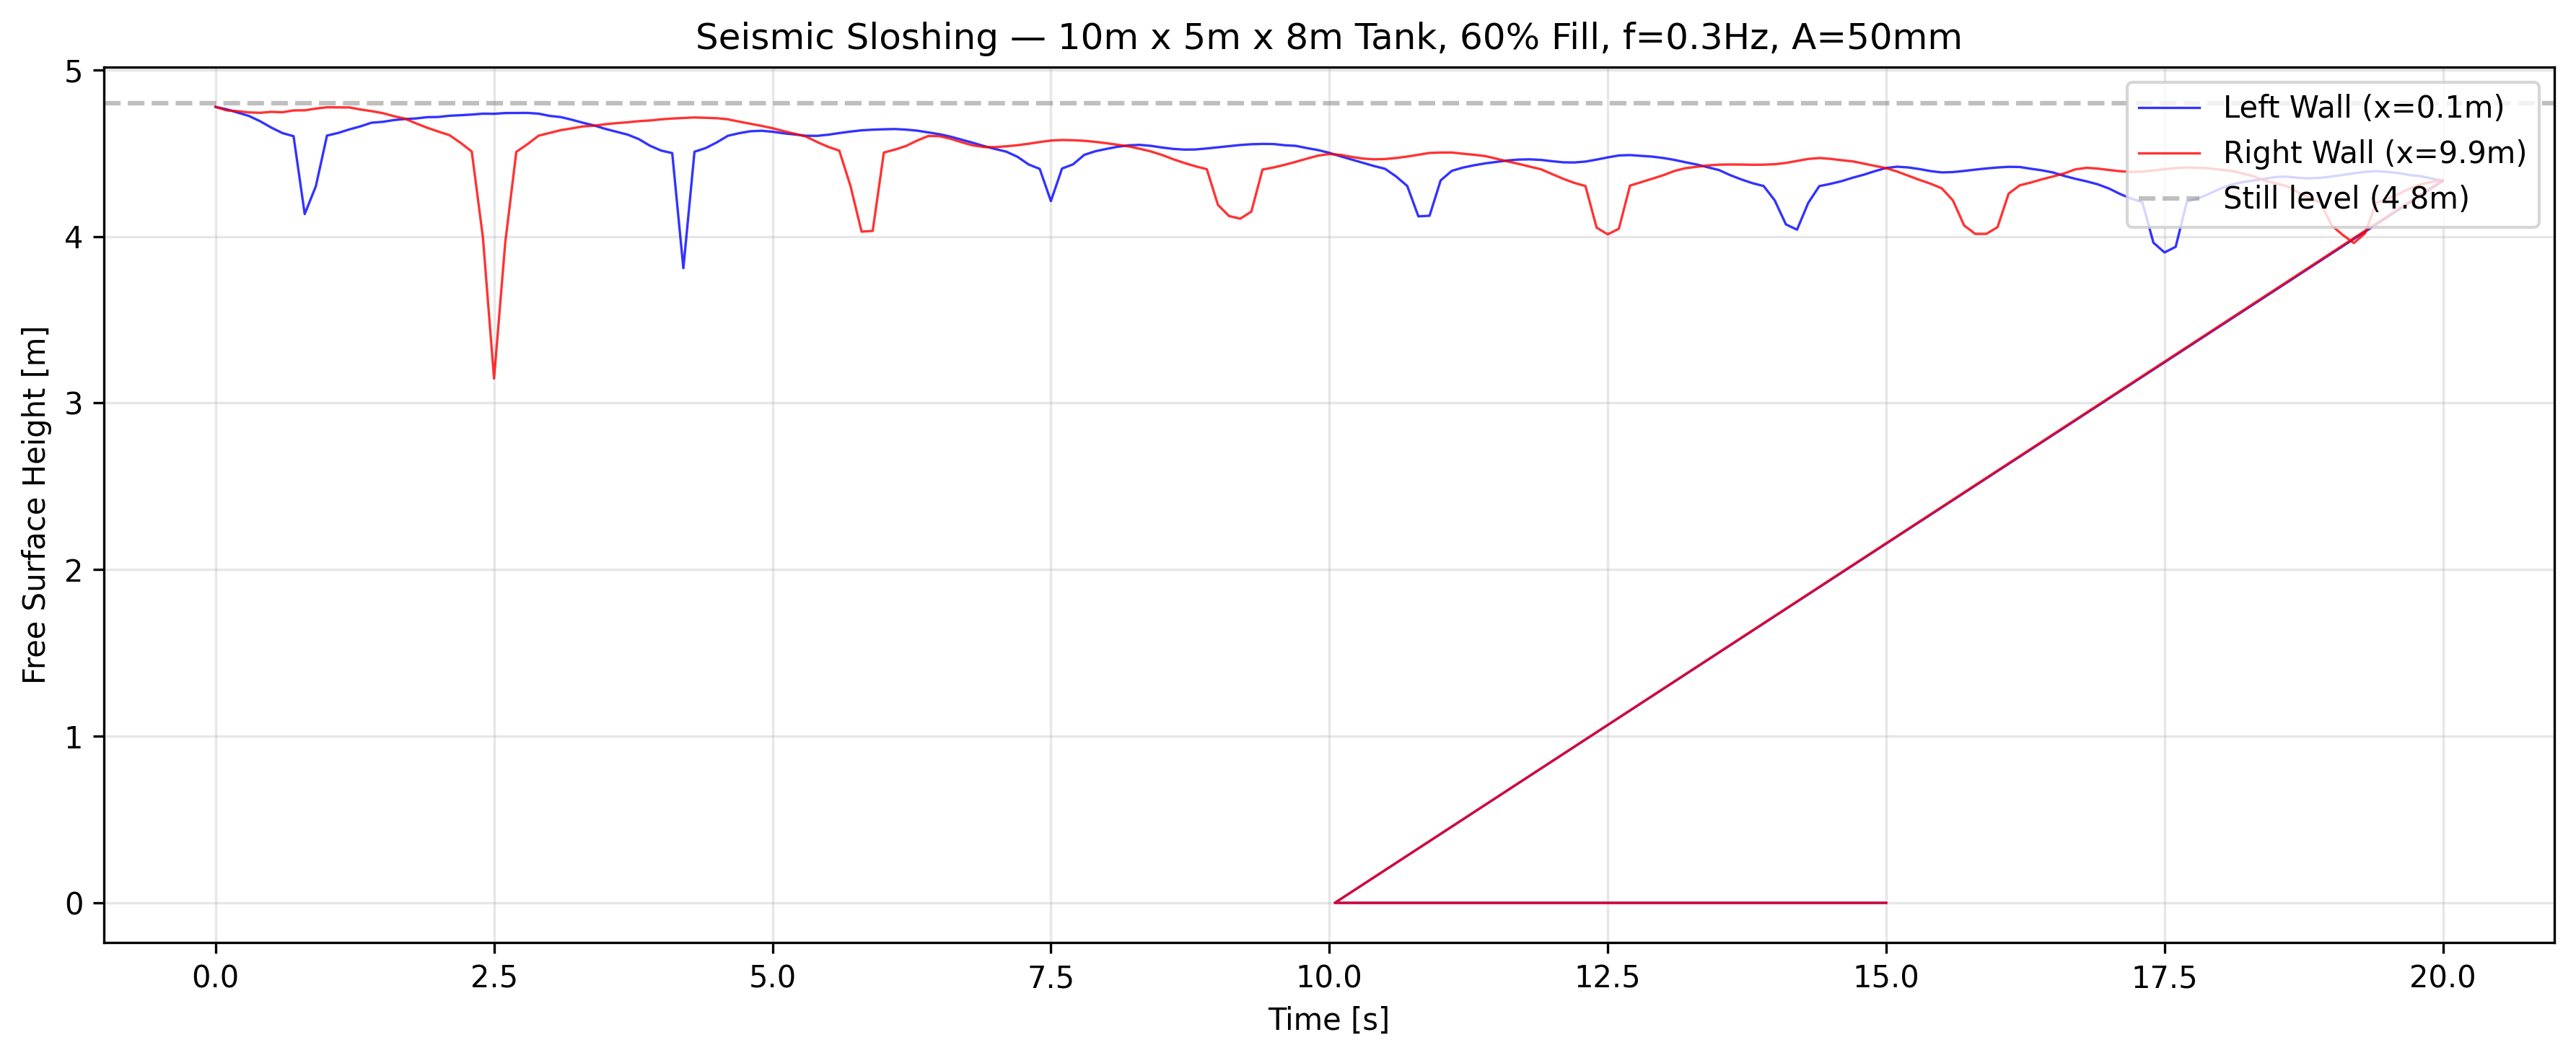
\includegraphics[width=\columnwidth]{../experiments/exp5_industrial/figures/fig6_seismic.png}
\caption{Seismic excitation scenario: petroleum storage tank under 0.3~Hz excitation showing extreme sloshing amplitude with complete wall drainage.}
\label{fig:seismic}
\end{figure}

The extreme amplitude (wave height exceeding the still-water level) and complete drainage at one wall indicate an overflow condition---physically correct for near-resonance large-tank excitation. This scenario illustrates the kind of industrial application (petroleum tank safety under earthquake loading) that motivates sloshing simulation automation~\citep{hatayama2004}.

\textbf{Both scenarios completed from single natural language prompts} without manual XML editing, demonstrating that SloshAgent can handle practical engineering design tasks beyond academic benchmarks.

\subsection{Summary of Key Findings}

Table~\ref{tab:key_findings} ranks the primary findings by novelty and evidence strength.

\begin{table}[htbp]
\centering
\caption{Summary of key findings ranked by novelty and evidence strength.}
\label{tab:key_findings}
\small
\begin{tabular}{@{}clp{3.8cm}p{3.2cm}@{}}
\toprule
\textbf{\#} & \textbf{Finding} & \textbf{Evidence} & \textbf{Statistical Support} \\
\midrule
1 & Complexity--accuracy boundary: L1+L2 accuracy 82\% vs L3+L5 8\% & EXP-2 & $p = 0.001$ (Mann--Whitney) \\
2 & First experimental benchmark validation: 7/7 water peaks within $\pm 2\sigma$ (non-normal dist.) & EXP-1 & All $|z| < 2.0$; Shapiro--Wilk $p < 0.005$ \\
3 & First domain knowledge ablation: FULL vs GENERIC medium effect ($d = 0.58$) on 32B & EXP-4 & $d = 0.58$; $p_{\text{bonf}} = 0.68$ (ns, $n = 10$) \\
4 & 32B vs 8B overall accuracy comparable (47\% vs 46\%) despite 32$\times$ latency difference & EXP-2 & $p = 0.715$ (Wilcoxon); latency $p < 0.001$ \\
5 & Model capacity threshold: domain prompt effect diverges ($d = 0.58$ vs $d = 0.15$) by model size & EXP-4 & Effect size comparison \\
6 & Parametric study reproduces 4/4 physical trends from Chen et al.\ (2018) & EXP-3 & Qualitative agreement \\
7 & 91.9\% baffle amplitude reduction in industrial PoC & EXP-5 & Demonstration \\
\bottomrule
\end{tabular}
\end{table}

% ============================================================
% 5. DISCUSSION
% ============================================================
\section{Discussion}

\subsection{Limitations}

We identify eight limitations that bound the generalizability of our findings.

\textbf{Single GPU hardware.} All experiments ran on a single NVIDIA RTX 4090 (24~GB VRAM), which limits practical particle counts to approximately 500K. Industrial LNG tank assessments at full scale may require millions of particles for converged pressure predictions~\citep{dominguez2022dualsphysics}. Multi-GPU or cluster-based execution---supported by DualSPHysics but not yet integrated into SloshAgent---would be required for production-scale deployments.

\textbf{Single LLM family.} All experiments used Qwen3 variants (32B and 8B) served via Ollama~\citep{qwen2025, ollama2024}. We did not evaluate proprietary models (GPT-4, Claude) or other open-weight families (Llama, Mistral). While the zero-cost local deployment is a design feature, the generalizability of our accuracy and ablation findings to other model architectures remains untested. CFD-Copilot~\citep{cfdcopilot2025} also uses Qwen3-32B for its general agent, suggesting this model class is competitive for simulation tasks, but direct cross-model comparison is needed.

\textbf{Solver-specific integration.} SloshAgent targets DualSPHysics v5.4 exclusively. The 14-tool interface assumes DualSPHysics-specific I/O patterns: XML case definition, GenCase preprocessing, binary particle output, and Run.csv telemetry. Other SPH solvers (SPHinXsys, GPUSPH) and mesh-based sloshing codes (OpenFOAM VOF) use different input formats and execution models. While we argue in Section~5.2 that the tool design patterns are transferable, this claim is not experimentally validated.

\textbf{DBC boundary limitation.} The oil sloshing failure in EXP-1 (zero detected impact peaks) is a documented limitation of the Dynamic Boundary Condition (DBC): its artificial viscosity over-damps low-energy viscous fluid impacts. English et al.~\citep{english2021mdbc} demonstrated that mDBC (modified DBC) resolves this issue. The current tool set does not support mDBC configuration, making viscous-fluid sloshing an open limitation.

\textbf{Moderate overall accuracy and sharp complexity boundary.} The 47\% parameter accuracy in EXP-2 (95\% CI [0.30, 0.67]) requires contextualization. The aggregate is driven down by L3 (paper-specific parameters absent from training data, 15\%) and L5 (edge cases requiring graceful refusal, 0\%). For standard use cases (L1 + L2), accuracy reaches 82\% (95\% CI [0.64, 0.95]). This complexity--accuracy boundary is statistically significant ($p = 0.001$) and delineates a clear practical envelope: SloshAgent handles explicit and domain-inference inputs reliably but is not a drop-in replacement for expert configuration at all complexity levels.

\textbf{Small-sample statistical power.} The ablation study (EXP-4, $n = 10$ scenarios per condition) produces a consistent directional ordering on 32B (FULL $>$ NO-RULES $>$ NO-DOMAIN $>$ GENERIC) with a medium effect size for the full-versus-generic comparison ($d = 0.58$). However, pairwise permutation tests do not reach significance after Bonferroni correction ($p_{\text{bonf}} = 0.68$). Larger-scale ablation studies with 30+ scenarios would be needed to confirm these directional findings at conventional significance thresholds. The 8B model shows no meaningful domain prompt benefit ($d = 0.15$, negligible), indicating that domain prompt engineering requires a minimum model capacity---a practical constraint for resource-limited deployments.

\textbf{No user study.} All evaluations are automated or expert-judged. The claim that SloshAgent makes sloshing simulation accessible to non-specialists is qualitative. A formal user study with naval architects or mechanical engineers who lack CFD expertise would be required to substantiate this claim.

\textbf{Incomplete quantitative validation.} The Chen2018 parametric study comparison (EXP-3) demonstrates physically consistent trends but lacks point-by-point quantitative validation against published figures, which would require figure digitization. The SPHERIC validation (EXP-1) uses the community-standard peak-within-band metric but does not report time-series correlation, which is inappropriate for sparse impact signals (see Section~4.2) but is sometimes expected by reviewers outside the sloshing community.

\subsection{From Sloshing to General Particle Simulation}

While SloshAgent is intentionally sloshing-specific, three of its design patterns generalize to the broader Lagrangian particle simulation ecosystem:

\textbf{IsError pattern for silent failure detection.} Particle solvers share a class of failures that produce output without error messages: divergent energy, particle leakage through boundaries, insufficient boundary layer thickness. SloshAgent's \texttt{error\_recovery} tool monitors Run.csv telemetry for anomalous kinetic energy growth and solver warnings. This pattern applies directly to DEM (Discrete Element Method) simulations, where particle overlap or explosive contact forces manifest as energy spikes, and to MPM (Material Point Method), where cell-crossing instabilities produce similar signatures.

\textbf{Asynchronous GPU job management.} The \texttt{job\_manager} and \texttt{monitor} tools implement a polling-based architecture that decouples the LLM reasoning loop from the GPU solver execution. This pattern is necessary for any GPU-accelerated particle solver where simulation times range from minutes to hours---far exceeding LLM API timeout windows. The same architecture would serve SPHinXsys (multi-physics SPH), LIGGGHTS (DEM for granular flow), and MPM solvers such as Taichi-MPM.

\textbf{Domain-encoded system prompts.} The EXP-4 ablation provides directional evidence (medium effect size, $d = 0.58$) that encoding domain physics (natural frequency formulas, fill-level sensitivity, parameter inference rules) into the system prompt improves generation accuracy on sufficiently large models (32B). While the small sample size ($n = 10$) limits statistical power, the consistent ordering and the contrasting negligible effect on 8B ($d = 0.15$) suggest that other particle simulation domains---powder processing (DEM), geomechanics (MPM), astrophysical SPH---may similarly benefit from domain-specific prompt engineering, provided the target LLM has sufficient capacity (32B+).

The broader implication is a ``particle-solver + LLM agent'' paradigm: any Lagrangian solver with a text-based input format, GPU execution, and domain-specific parameter constraints is a candidate for LLM agent automation using the patterns established here.

\subsection{Industry Impact Projection}

SloshAgent's practical value is best understood against the economics of current sloshing analysis workflows.

\textbf{Time reduction.} A single sloshing case requires expert-level XML authoring (1--4 hours depending on complexity), solver execution (minutes on GPU), and result interpretation. SloshAgent reduces the authoring phase to a single natural language prompt (seconds to minutes of LLM inference). For the 200+ case parametric studies required for LNG tank certification~\citep{isope2012sloshing}, this compression from months of expert effort to days of automated execution represents a qualitative shift in workflow efficiency.

\textbf{Cost structure.} SloshAgent operates at zero marginal LLM cost: Qwen3 32B runs locally via Ollama on consumer-grade hardware. Combined with DualSPHysics (open-source, GPU-accelerated), the entire stack avoids both cloud API fees (\$0.01--0.06 per 1K tokens for proprietary models) and commercial solver licenses (\$10K+/year). By contrast, CFD consulting rates of \$80--120/hour and project costs of \$2K--20K per study~\citep{cadcrowd2024} create significant barriers for iterative design exploration. BCG projects that AI-assisted R\&D can deliver 10--20\% time-to-market reduction and up to 20\% cost reduction~\citep{bcg2025}.

\textbf{Reproducibility advantage.} All components of the SloshAgent stack are open: DualSPHysics (LGPL), Qwen3 (Apache 2.0), and SloshAgent itself. This contrasts with systems that depend on proprietary APIs (MetaOpenFOAM on GPT-4o~\citep{metaopenfoam2024}, ChatCFD on DeepSeek~\citep{chatcfd2026}), where reproducibility is contingent on API availability and pricing stability.

% ============================================================
% 6. CONCLUSION
% ============================================================
\section{Conclusion}

Sloshing---the violent motion of liquid in partially filled containers---causes catastrophic failures across aerospace, maritime, petrochemical, nuclear, and transportation industries, with cumulative documented damages exceeding \$15~billion. Predicting sloshing loads requires over 200 simulations per LNG tank design, each demanding expert-level configuration of specialized solvers. Despite a \$4.13~billion maritime AI market, no AI system has previously automated any part of this workflow.

This paper presented SloshAgent, to our knowledge the first AI agent that automates the entire sloshing simulation pipeline---from natural language input to experimentally validated results---using DualSPHysics, the leading open-source GPU-accelerated SPH solver. We summarize five contributions, each linked to experimental evidence:

\textbf{First sloshing simulation automation agent (EXP-2).} SloshAgent converts natural language descriptions into valid DualSPHysics XML configurations with 85\% tool call success and 70\% physical validity across 20 scenarios at five complexity levels. A statistically significant complexity--accuracy boundary ($p = 0.001$) separates standard use cases (L1+L2: 82\%, 95\% CI [0.64, 0.95]) from paper-specific and edge cases (L3+L5: 8\%). The two model sizes (32B and 8B) achieve comparable overall accuracy ($p = 0.715$).

\textbf{First LLM agent for particle-based simulation (Architecture).} We designed 14 domain-specific tools covering the complete DualSPHysics pipeline---to our knowledge, the first tool interface for any Lagrangian particle solver (SPH, DEM, or MPM)---including an IsError pattern for LLM self-correction of silent SPH failures and asynchronous GPU job management.

\textbf{First experimental benchmark validation by an LLM-simulation agent (EXP-1).} Agent-generated SPHERIC Test~10 simulations reproduce all detected water impact pressure peaks within the $\pm 2\sigma$ experimental scatter band (7/7 peaks, all $|z| < 2.0$), following the standard SPHERIC/ISOPE validation protocol. The non-normal experimental distribution (Shapiro--Wilk $p < 0.005$, CV = 20--36\%) confirms that band-based validation is the appropriate metric for stochastic impact flows. The oil case failure (DBC boundary limitation) is an honest solver constraint, not an agent deficiency.

\textbf{First domain prompt ablation for computational mechanics (EXP-4).} A four-condition ablation of the 136-line SloshingCoderPrompt reveals a medium effect size ($d = 0.58$) for domain knowledge encoding on the 32B model, with a consistent ordering FULL $>$ NO-RULES $>$ NO-DOMAIN $>$ GENERIC. The contrasting negligible effect on 8B ($d = 0.15$) and the observed inversion (FULL underperforms NO-RULES) reveal a model capacity threshold for effective prompt engineering. Larger-scale studies are needed to confirm these directional findings at conventional significance levels.

\textbf{Industry proof-of-concept at zero LLM cost (EXP-3, EXP-5).} Automated parametric studies (six fill levels from a single prompt, reproducing four physical trends from Chen et al.\ (2018)) and industrial scenarios (91.9\% baffle amplitude reduction, seismic tank excitation) demonstrate practical applicability. The entire stack runs on local hardware (Qwen3 32B via Ollama, RTX 4090) with no cloud API dependencies.

\textbf{Future work.} Four directions emerge from this study. First, multi-solver integration (SPHinXsys, OpenFOAM VOF) would test the generalizability of the tool interface patterns beyond DualSPHysics. Second, a formal user study with naval architects and mechanical engineers would validate the non-expert accessibility claim. Third, lightweight fine-tuning or retrieval-augmented generation could address the L3 (paper-specific) and L5 (edge case) accuracy gaps without increasing prompt length. Fourth, an LNG industry pilot with classification society involvement would bridge the gap between academic validation and production deployment.

% ============================================================
% BIBLIOGRAPHY
% ============================================================
\bibliographystyle{plainnat}
\bibliography{../references}

\end{document}
